%!TEX program = xelatex
\documentclass[twocolumn]{jbuaa}

%将\newcommand 和 \usepackage 全部写入 jbuaa。cls文件中方便管理
%\citeBUAA{Anonymous:2017jp} 为引用格式(当你引用的时候自动设置序号和参考文献)
%{Anonymous:2017jp},{}里面写的标签是bib文件中,每一篇论文都会有一个



\begin{document}

	% % 这一行用来去掉默认的日期显示   和标题
	\title{}
	\date {}  

	\twocolumn[
		\begin{@twocolumnfalse}
			\maketitle %显示标题(目的是为了显示第一页的页眉设置)

			\begin{flushleft}
				\vspace{-22mm}%为了调高标题位置

				\parbox{\textwidth}{
					\setlength{\parindent}{0em}{
						\sihao\textbf{包含逆向物流的无人机路径规划} \xiaowuhao\fang \\
					} \vspace{-2mm}%行距(标题与作者之间的距离)

					\begin{flushleft}
						%英文作者(和中文设置一样)
						{\wuhao 沈天马\makebox{$^{\text{1}}$}}\\[0.2cm]
						\liuhao{(1.~~上海理工大学大学~~光电信息与计算机工程学院,上海~~200930;)}
						% {\wuhao Tian-ma Shen\makebox{$^{\text{1}}$}, LI Mou\makebox{$^{\text{1,2,*}}$}, SHANGGUAN Moumou\makebox{$^{\text{2,3}}$}, LIN Mou\makebox{$^{\text{3}}$}, ZHAO Mou\makebox{$^{\text{3}}$}, WANG Mou\makebox{$^{\text{3}}$}}\\[-0.1cm]
						% \liuhao{(1. School of Aeronautic Science and Engineering, Beijing University of Aeronautics and Astronautics, Beijing 100191, China;\\
						% 2. School of Astronautics, Beijing University of Aeronautics and Astronautics, Beijing 100191, China;\\
						% 3. College of Automation, Northwestern Polytechnical University, Xi’an 710072, China)}
					\end{flushleft}\vspace{3mm}%调整行距					
				}
			\end{flushleft}
				%关键字
			\CKeyword{无人机; 逆向物流;动态规划;K-Means聚类;TSP旅行商问题;遗传算法}
			%中图分类号
			\CLCNo{V221\makebox{$^{\scalebox{0.6}{\!+}}$}.3;TB553}
			%文献标识码
			\Dcode{A}
			%文章编号
			\PaperNo{1001-5965 (XXXX) XX-XXXX-XX}

			%标题上方的信息
			% \positiontextbox{2.2cm}{2.9cm}{\wuhao http://bhxb.buaa.edu.cn \quad  jbuaa@buaa.edu.cn\\[0.3cm]
			% \wuhao DOI: \ 10.13700/j.bh.1001-5965.****.****}

			%%%%%%%%%%%%%%%%%%%%%%%%%%%%%%%%%%%%%%%%%%%%%%%%%%%%%%%%%%%%%%%%
			%      中文摘要
			%%%%%%%%%%%%%%%%%%%%%%%%%%%%%%%%%%%%%%%%%%%%%%%%%%%%%%%%%%%%%%%%
			\begin{CAbstractJBUAA}
				近年来,国内外大型自营物流企业,如亚马逊、京东等,开始研究无人机路径规划。并且随着城市的不断发展,逆向物流在传统物流中的比重不断提高,加剧了物流路径规划的难度。通过对无人机路径规划的研究和逆向物流的分析,提出了一种基于K-Means聚类算法、遗传算法的动态规划模型。根据企业的不同情况,将逆向物流也融入到传统物流路径之中,并且企业可以针对不同地区、不同时期的条件下建立仿真模型,提前合理分配不同地域无人机数量的调度问题,将物流成本降到最低。对于某一配送区域,先通过带权值的K-Means算法,将该区域划分成K簇,每一簇分配一架无人机。即对应不同数量、位置、大小和重量包裹,通过加权聚类来确定无人机最小数量。其次对每一簇路径的规划问题转化为TSP旅行商问题。在每一簇坐标数据对应的连通图中,通过遗传算法对可行解进行编码,从而求解出最小欧拉回路,即近似最优路径。
			\end{CAbstractJBUAA}

			%%%%%%%%首页角注,{2.0cm}{27cm}以左上方为坐标原点
			\positiontextbox{2.0cm}{27.4cm}{
				\noindent\rule{4cm}{.5pt}\\[0.5ex]%
				\hspace*{1em} \liuhao \linespread{0.8}\selectfont
				\parbox{\textwidth}{%
				% \hei\makebox[\widthof{\makebox{*}收}][r]{收}稿日期: 2015-**-**; 录用日期: 2015-**-**; 网络出版时间:(此行信息已填) \\%
				% \hei\makebox[\widthof{\makebox{*}收}][r]{网}络出版地址: (已填)\\
				% \hei\makebox[\widthof{\makebox{*}收}][r]{基}金项目:国家自然科学基金(基金号~12345678);中国博士后科学基金(基金号~87654321)(注意:国家级基金放前,地方级放后)\\
				% \hei\makebox[\widthof{\makebox{*}收}][r]{\makebox{*}通}信作者:E-mail:bhxb@buaa.edu.cn\\ \\
				% \hei\makebox[\widthof{\makebox{*}收}][r]{引}用格式:(可不填)
				}
			}


			%%%%%%%%%%%%%%%%%%%%%%%%%%%%%%%%%%%%%%%%%%%%%%%%%%%%%%%%%%%%%%%%
  			%          英文摘要
  			%%%%%%%%%%%%%%%%%%%%%%%%%%%%%%%%%%%%%%%%%%%%%%%%%%%%%%%%%%%%%%%%
			\begin{flushleft}
				\parbox{\textwidth}{

					%英文标题
					\setlength{\parindent}{0em}{%0em 让摘要前不空格
						\sihao\textbf{UAV Reverse Logistics Dynamic Physical Network Design} \xiaowuhao\fang \\
					} \vspace{-2mm}%行距(标题与作者之间的距离)

					\begin{flushleft}
						%英文作者(和中文设置一样)
						{\wuhao Shen Tian-ma \makebox{$^{\text{1}}$}}\\[0.2cm]
						\liuhao{(1. University of Shanghai for Science and Technology, Shanghai, 200930 ,P.R.China)}
						% {\wuhao Tian-ma Shen\makebox{$^{\text{1}}$}, LI Mou\makebox{$^{\text{1,2,*}}$}, SHANGGUAN Moumou\makebox{$^{\text{2,3}}$}, LIN Mou\makebox{$^{\text{3}}$}, ZHAO Mou\makebox{$^{\text{3}}$}, WANG Mou\makebox{$^{\text{3}}$}}\\[-0.1cm]
						% \liuhao{(1. School of Aeronautic Science and Engineering, Beijing University of Aeronautics and Astronautics, Beijing 100191, China;\\
						% 2. School of Astronautics, Beijing University of Aeronautics and Astronautics, Beijing 100191, China;\\
						% 3. College of Automation, Northwestern Polytechnical University, Xi’an 710072, China)}
					\end{flushleft}\vspace{2.3mm}%调整行距

					%          英文摘要
					\vspace{-10pt}\wuhao{
						%          英文摘要
						\textbf{Abstract:} 
						In recent years, domestic and foreign large-scale self-supporting logistics companies such as Amazon and Jingdong started to study UAV path planning. And with the continuous development of the city, the proportion of reverse logistics in the traditional logistics continues to increase, exacerbating the difficulty of the logistics path planning. Through the research of UAV path planning and reverse logistics analysis, a dynamic programming model based on K-Means clustering algorithm and genetic algorithm is proposed. According to the different circumstances of enterprises, the reverse logistics will also be integrated into the traditional logistics path, and enterprises can set up simulation models for different regions and different periods under the conditions of reasonable distribution in advance, the number of UAV scheduling in different regions, the logistics costs drop to lowest. For a certain distribution area, the area is divided into K clusters by weighted K-Means algorithm and each cluster is assigned a UAV. That is, corresponding to different number, location, size and weight of the package, through the weighted clustering to determine the minimum number of UAVs. Secondly, the planning problem of each cluster path is transformed into the TSP traveling salesman problem. In the connected graph corresponding to each cluster coordinate data, the feasible solution is encoded by genetic algorithm to solve the minimum Euler circuit, that is, the approximate optimal path.

						%英文关键字
						\textbf{Key words:} reverse logistics, dynamic physical network design, K-Means cluster, genetic algorithm, Travelling Salesman Problem 
					}
				}
			\end{flushleft}
		\end{@twocolumnfalse}
	]

	%%%%%%%%%%%%%%%%%%%%%%%%%%%%%%%%%%%%%%%%%%%%%%%%%%%%%%%%%%%%%%%%
	%  正文由此开始-------------------------
	%%%%%%%%%%%%%%%%%%%%%%%%%%%%%%%%%%%%%%%%%%%%%%%%%%%%%%%%%%%%%%%%
	%%%%%%%%%%%%%%%%%%%%%%%%%%%%%%%%%%%%%%%%%%%%%%%%%%%%%%%%%%%%%%%%
	\wuhao 
	%  分栏开始

	%%%%%!!!!!正文在第一页两栏分别合适位置插入 \enlargethispage{-3.3cm},给首页跨双栏脚注留空间,大小需要结合前面位置和高度手动设置!!!!!
	%%%%%%%%%%%%%%%%%%%%%%%%%%%%%%%%%%%%%%%%%%%%%%%%%%%%%%%%%%%%%%%%

	\enlargethispage{-3.3cm}
	\section{引言}
	逆向物流的需求不断提高,给国内外自营物流企业的物流配送成本急剧上升。包含逆向物流动的无人机态路径规划模型的进入,可以给物流厂商在商业领域的成本问题带来巨大的收益。无人机是一种通过动力驱动的无人驾驶、可重复使用的飞行器(Unmanned Aerial Vehicle,UAV)\citeBUAA{Lin:2017dz}。虽然无人机很早的进入普通民众的视野,但是在2013年之前却无人将无人机技术应用到物流配送领域。2013 年 9
	月,国内物流公司顺丰速运首次进行了无人机派件测试;2013年12月初,美国电商巨头亚马逊公司和联合包裹运送服务公司(UPS)先后宣布启动无人机配送项目;2015年11月,亚马逊向媒体公开展示最新一代无人机Prime Air drone;2016年5月,国内大型自营物流电商京东也推出两款无人机,分别是垂直起降固定翼无人机和三轴六旋翼无人机\citeBUAA{:2015jp}。无人机商用现象并非个案,实际上,DHL、淘宝菜鸟物流、圆通等企业都测试或构想无人机运送方案。物流公司都认识到,启用无人机投递快件能够缩短客户从订货到签收的时间,并且无人机具有垂直起降、起飞着陆场地小、空中悬停、机动灵活、任务能力广泛、造价低等功能特点和应用优势\citeBUAA{:2017kd}。
	%\citeBUAA{Anonymous:2017jp} 为引用格式(当你引用的时候自动设置序号和参考文献)
	%{Anonymous:2017jp},{}里面写的标签是bib文件中,每一篇论文都会有一个
	%
	\\\indent{}美国物流管理协会对于逆向物流的概念是: 为了资源回收以及处理废弃物,在有效及适当成本下,对原材料、在制品、成品和相关信息,从消费 点到原始出产点的流动和储存进行规划、执行与管 理的过程,从而达到回收价值和适当处置的目的\citeBUAA{deBrito:2003hv}。在物流的逆向过程中,物流具有更多的复杂性和不确定,给当代物流企业带来不小的额外物流成本。所以在近10年中,逆向物流收到了越来越多企业的重视。\citeBUAA{Sangwan:2017ex}为了针对其不确定性,本文模型需考虑到动态性,能及时的对突发的逆向需求做出调整,得到全新的最优路径。针对其复杂度,本文模型把配送点的坐标数据映射到连通图中,将问题转化为TSP旅行商问题\citeBUAA{Hoffman:2001el},运用一种特殊字符编码型的遗传算法求解模型最优解,有效避免算法迭代过程中奇异解的产生,得出每架无人机的飞行最优派送路径。在设计模型是还需要考虑到无人机的性能指标,如最大飞行速度60千米/小时,铅垂面内最大加速±2米/秒$^{2}$,最大续航时间为2小时,飞行时的转弯半径不小于100米,最大爬升(俯冲)角度为±15°,与其它障碍物(含地面)的安全飞行距离不小于50米,最大飞行高度为海拔1000米。
	\enlargethispage{-3.3cm}












	\section{动态规划模型}
	% \enlargethispage{-3.3cm}

	\subsection{加权归一化}

	对于配送包裹有不同数量、位置、体积和重量这四个特征属性,所以只考虑坐标数据对其聚类太过于片面化。因此将其数量、体积、重量和正逆向这四个数值加权后的结果,作为坐标数据的加权系数,从而解决不同坐标下权重分配问题。数量、体积、重量的单位、物理意义和定义域的范围都各不相同,所以在数值加权前必须进行归一化处理,解决数据不统一问题。考虑到三个数据的物理意义直接将其映射到$[0,1]$区间,式(1)。
	%
	\begin{eqnarray}
		\overline {X^{\left( i\right) }_{j}}&=&\frac {X^{\left( i\right) }_{j}-\min }{\max -\min }
	\end{eqnarray}
	%
	\\\indent{}其中$\max$为$X_{j}$定义域内的最大值;$\min$为$X_{j}$定义域内的最小值;$X_{1}$为包裹的数量;$X_{2}$为包裹的体积;$X_{3}$为包裹的重量;$X_{4}$为正向或逆向物流。
	\\\indent{}经过归一化处理后,得到单位统一的特征属性值$\overline {X^{\left( i\right) }_{j}}$,对其做线性加权,式(2),得到每一个包裹对应的加权系数$\overline {W^{\left( i\right) }}$。
	%
	\begin{eqnarray}
		\overline {W^{\left( i\right) }}&=&\sum _{j}W_{j}\cdot \overline {X^{\left( i\right) }_{j}}
	\end{eqnarray}
	%
	\\\indent{}其中$W_{j}$为对应特征属性$X_{j}$的加权系数。
	%
	%
	%
	\begin{figure*}[!h]

		\centering                                             %居中
		\subfigure[]{                                          %第一张子图
		\begin{minipage}{5cm}
		\centering                                           %子图居中
		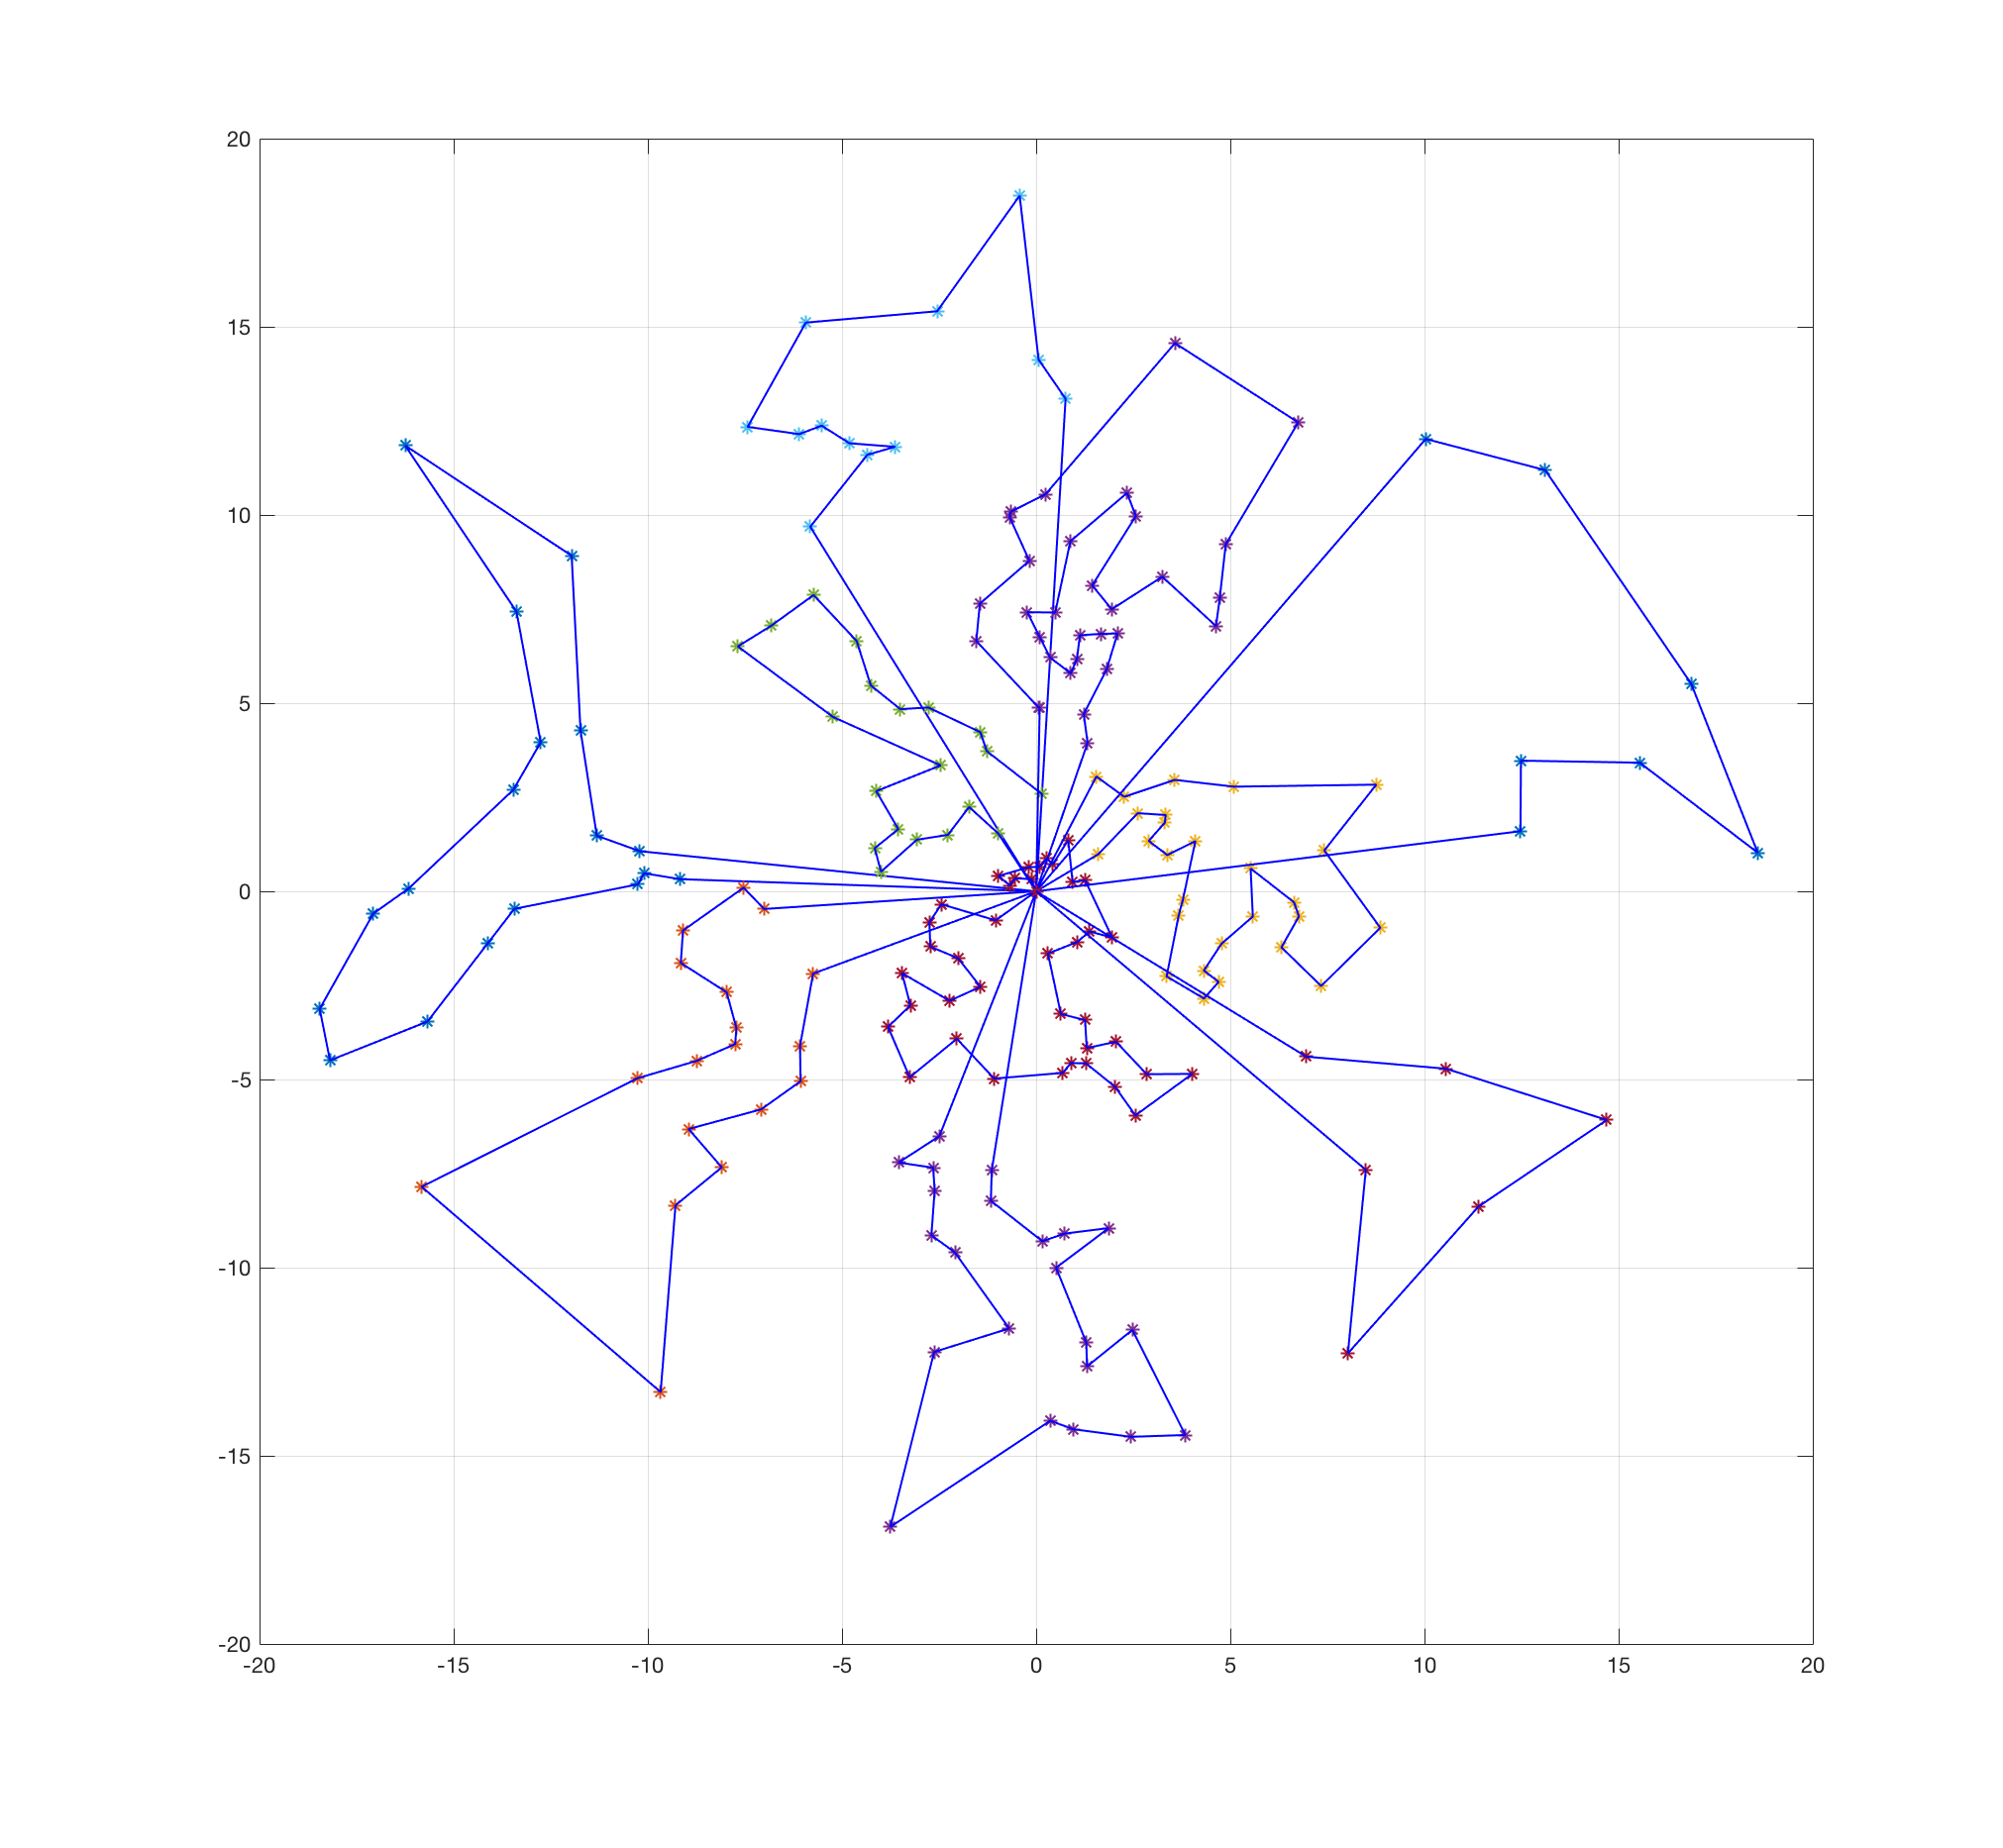
\includegraphics[scale=0.08]{Figs/uav1000_1.png}             
		\end{minipage}}
		%
		%第二张子图
		\subfigure[]{                    
		\begin{minipage}{5cm}
		\centering                        %子图居中
		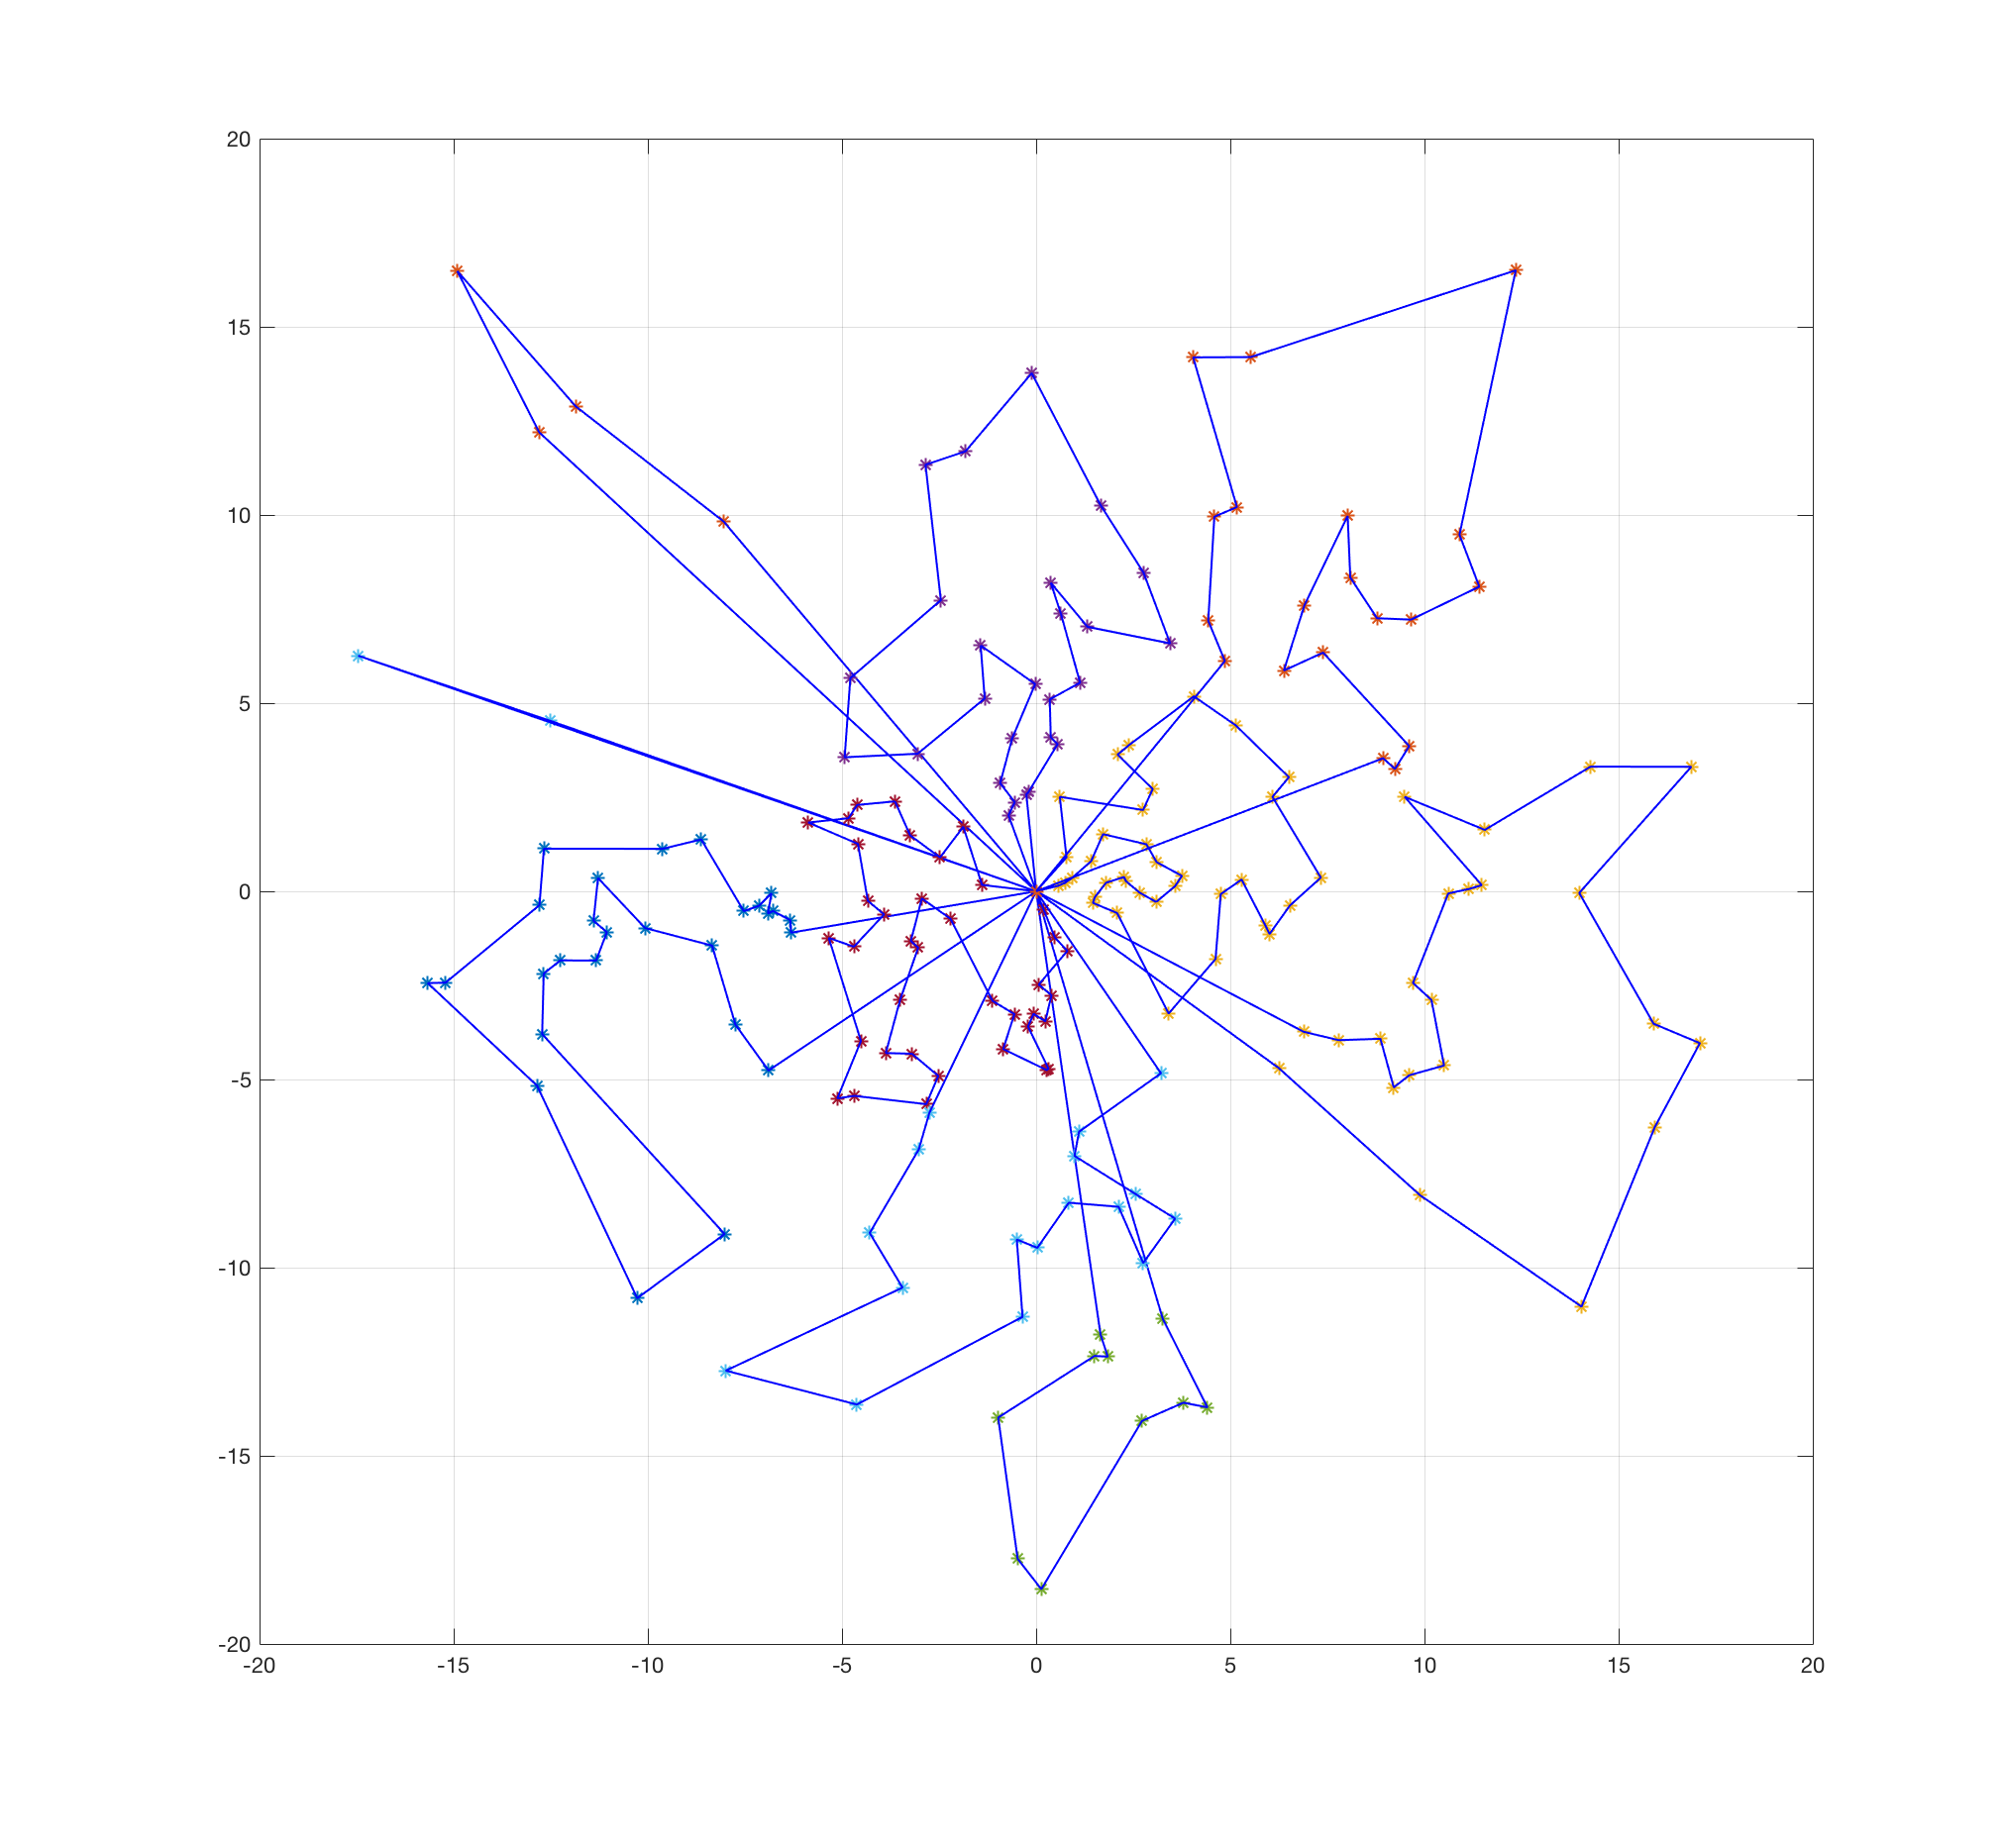
\includegraphics[scale=0.08]{Figs/uav1000_2.png}             
		\end{minipage}}
		%
		%第3张子图
		\subfigure[]{                    
		\begin{minipage}{5cm}
		\centering                        %子图居中
		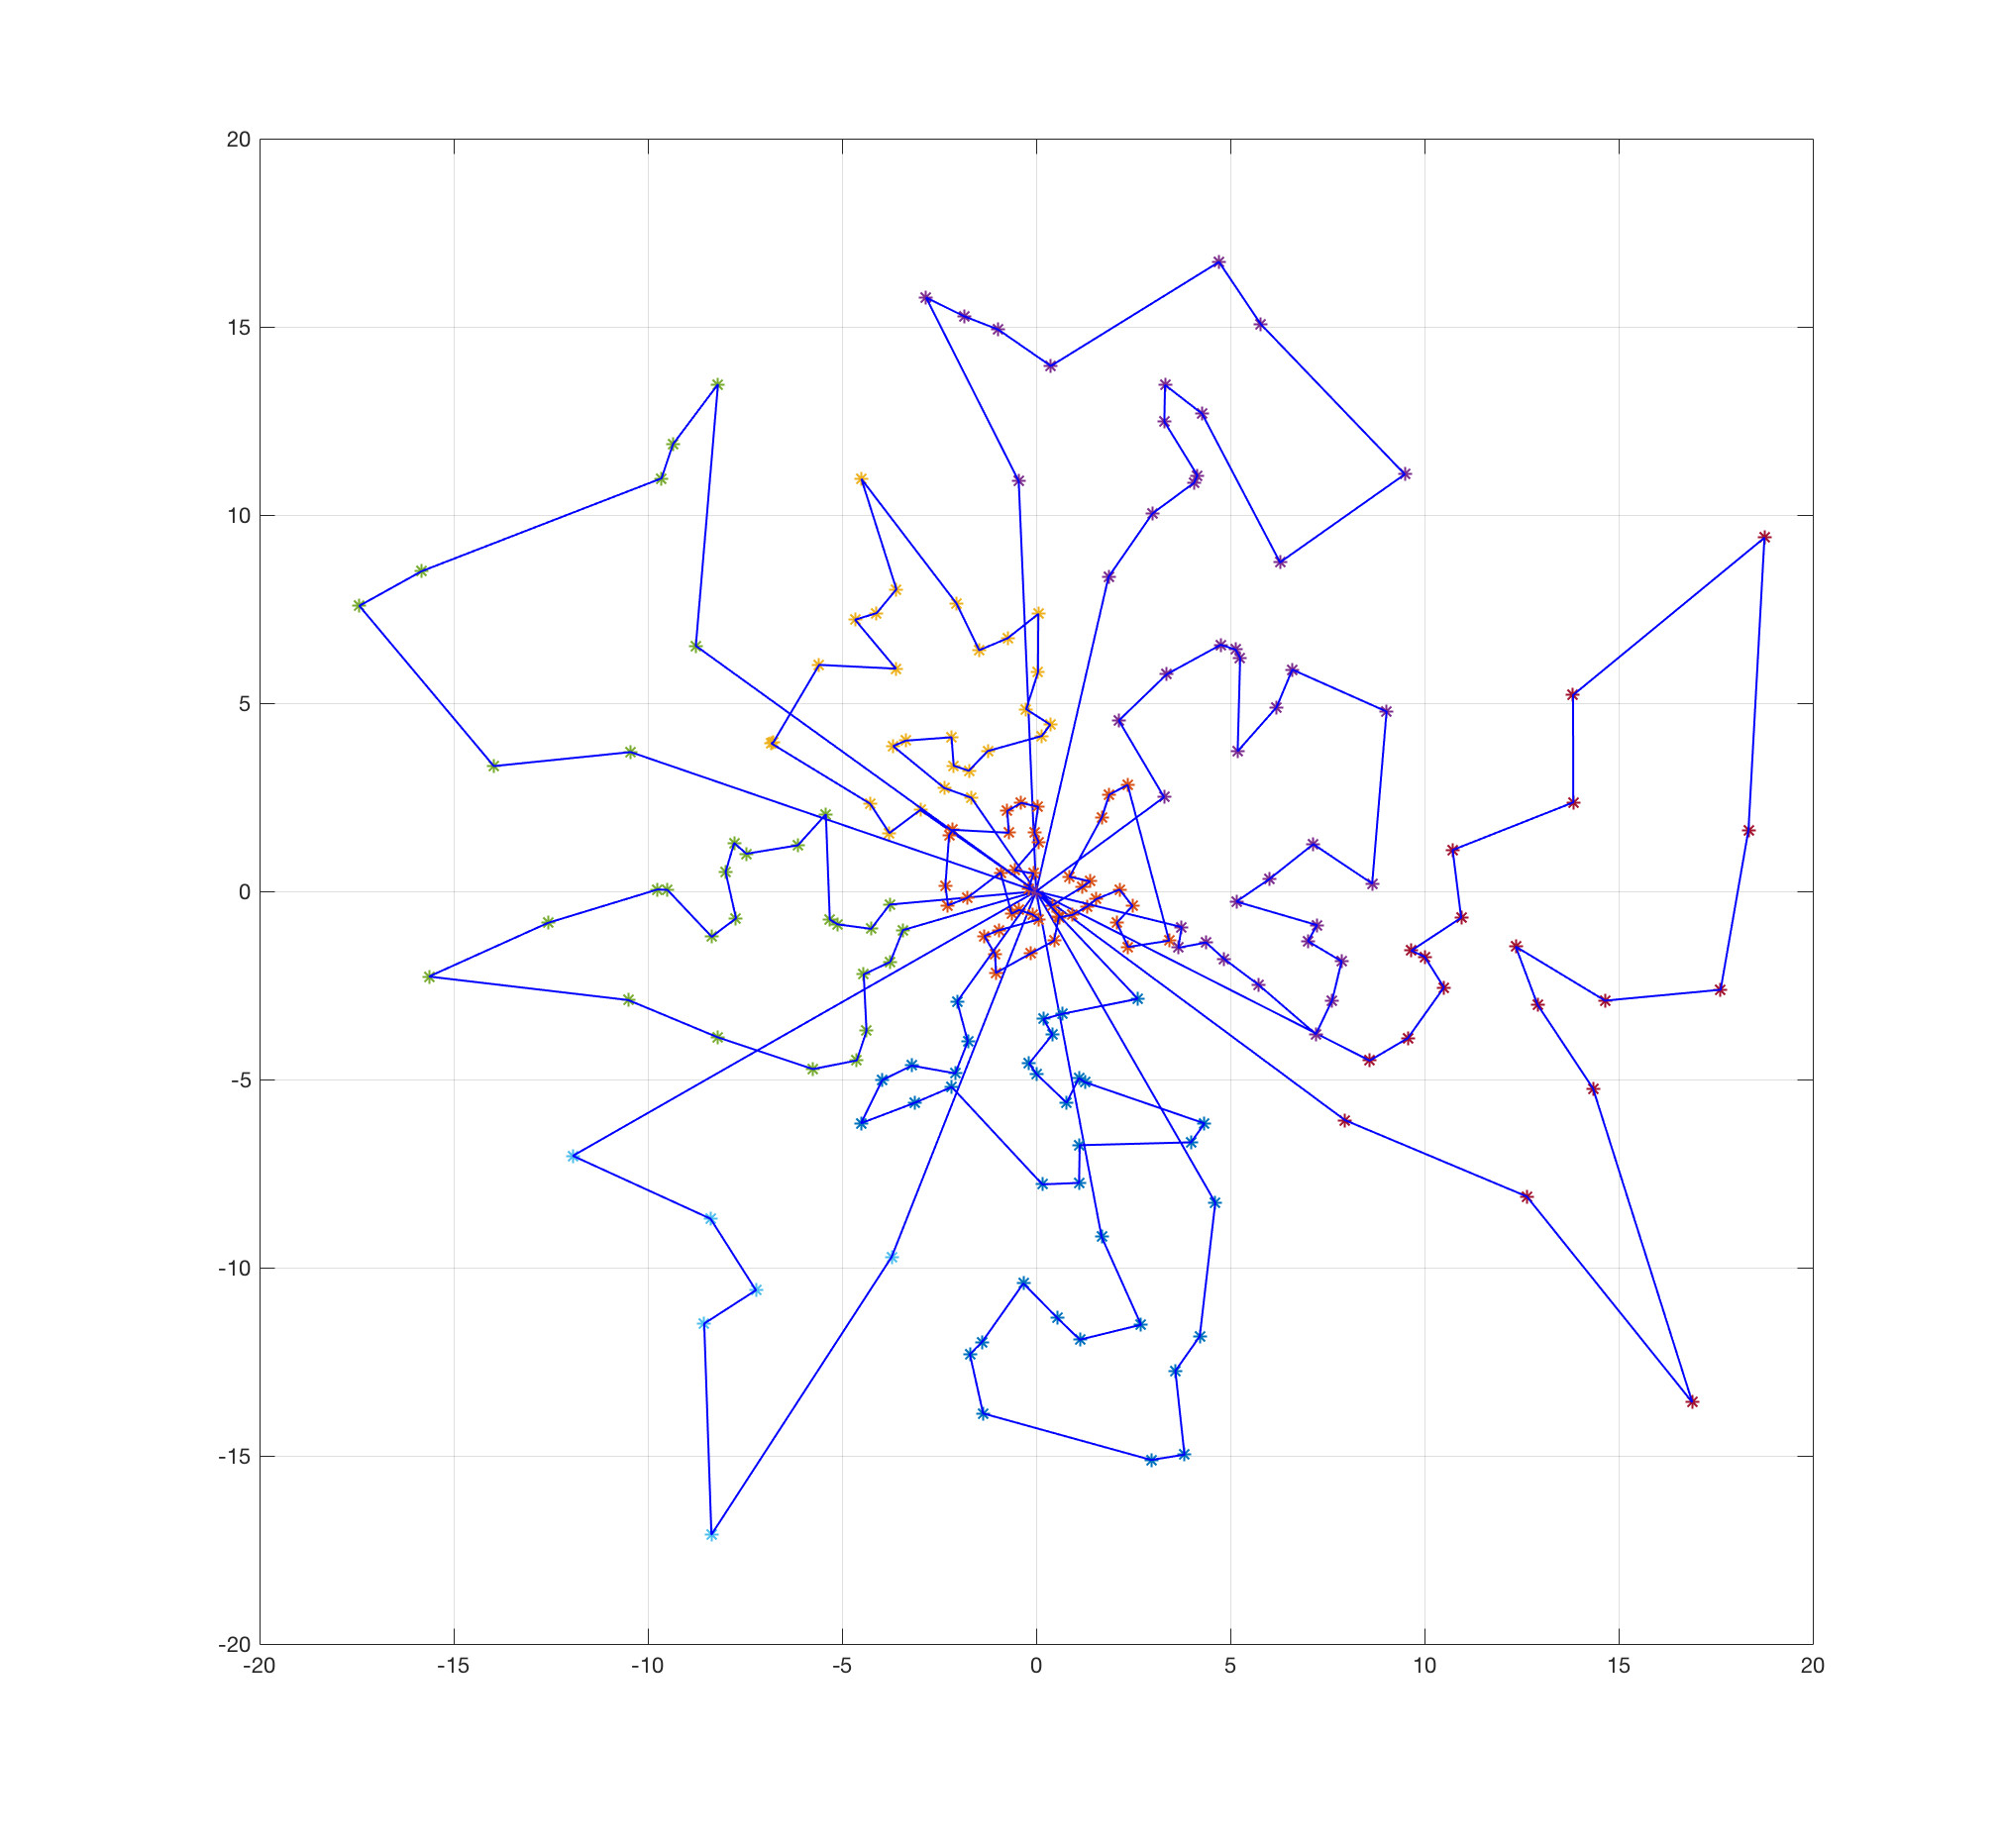
\includegraphics[scale=0.08]{Figs/uav1000_3.png}             
		\end{minipage}}
		% %
		% %第4张子图
		% \subfigure[]{                    
		% \begin{minipage}{6cm}
		%   \centering                        %子图居中
		%   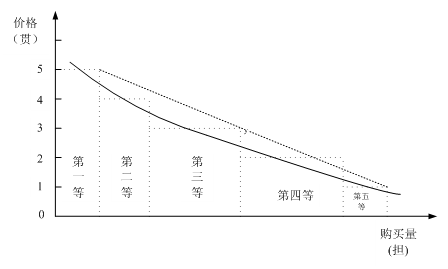
\includegraphics[scale=0.4]{Figs/01.png}             
		% \end{minipage}}
		%                                           
		%大图名称
		\caption{包裹量$N$为1000时,不同随机产生数据下动态规划路线结果图(3幅)} 
		\label{fig:3}                                          %图片引用标记

	\end{figure*}


	\begin{figure*}[!h]

		\centering                                             %居中
		\subfigure[]{                                          %第一张子图
		\begin{minipage}{5cm}
		\centering                                           %子图居中
		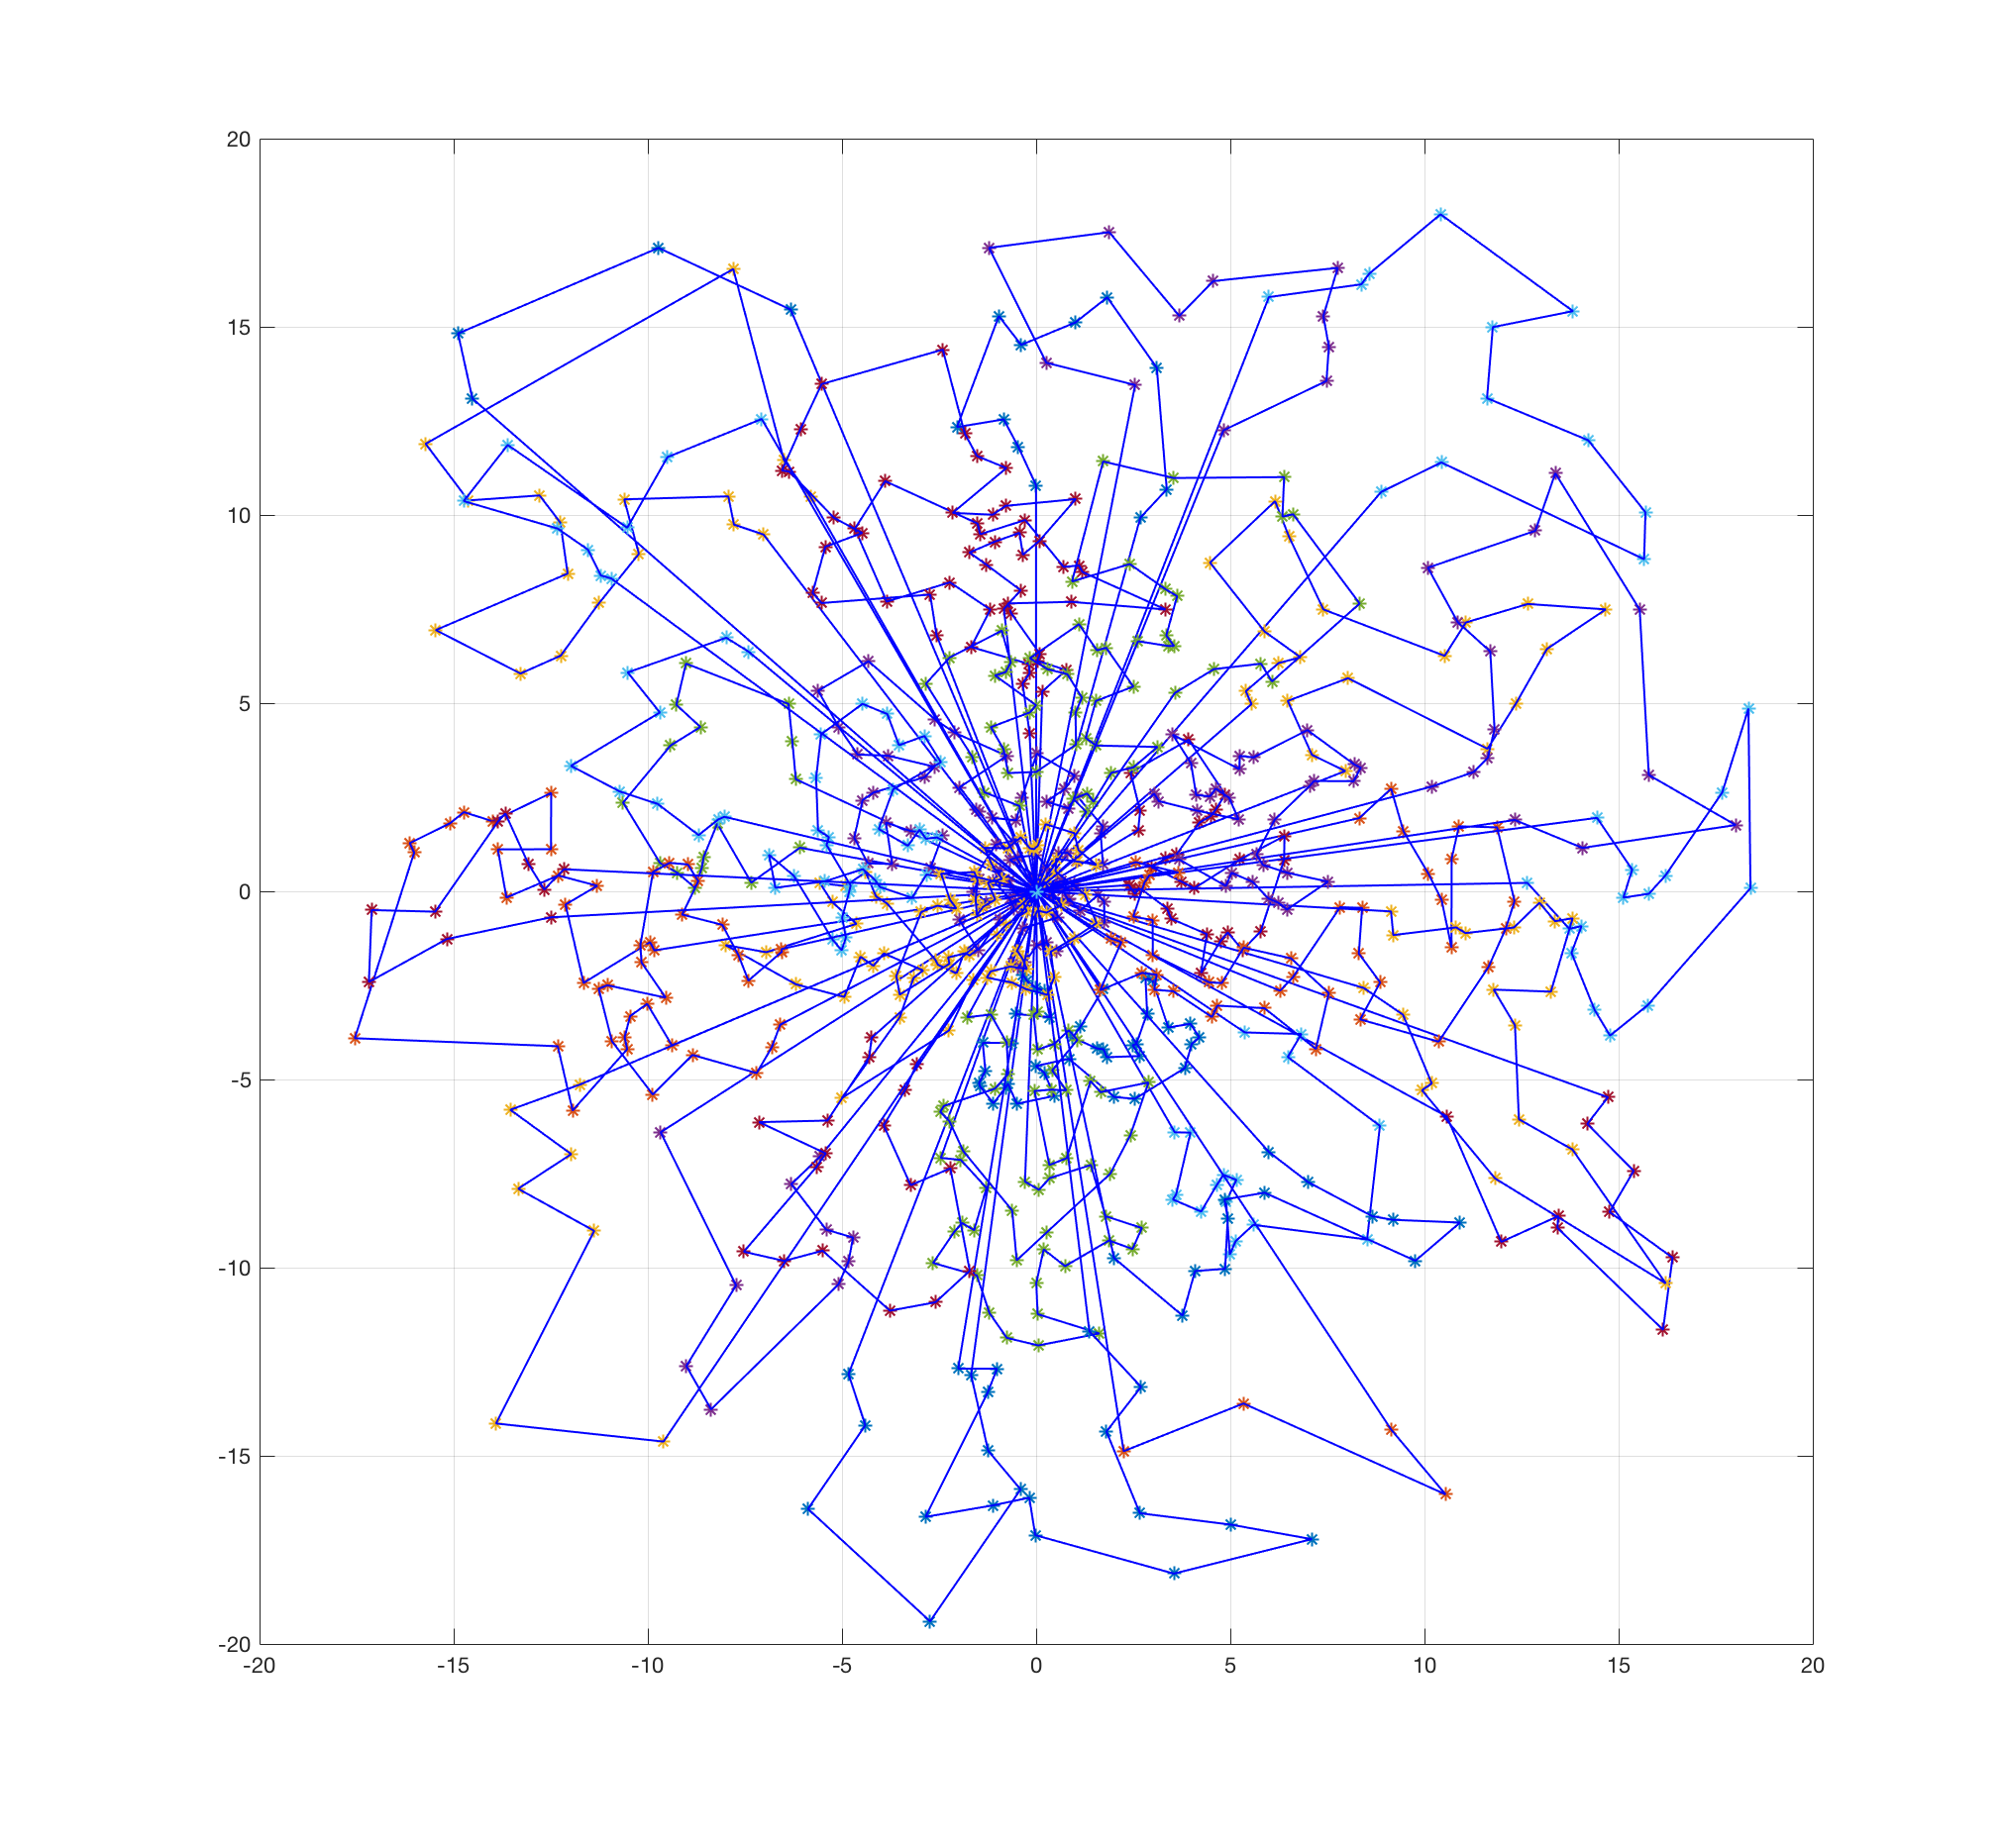
\includegraphics[scale=0.08]{Figs/uav8000_1.png}             
		\end{minipage}}
		%
		%第二张子图
		\subfigure[]{                    
		\begin{minipage}{5cm}
		\centering                        %子图居中
		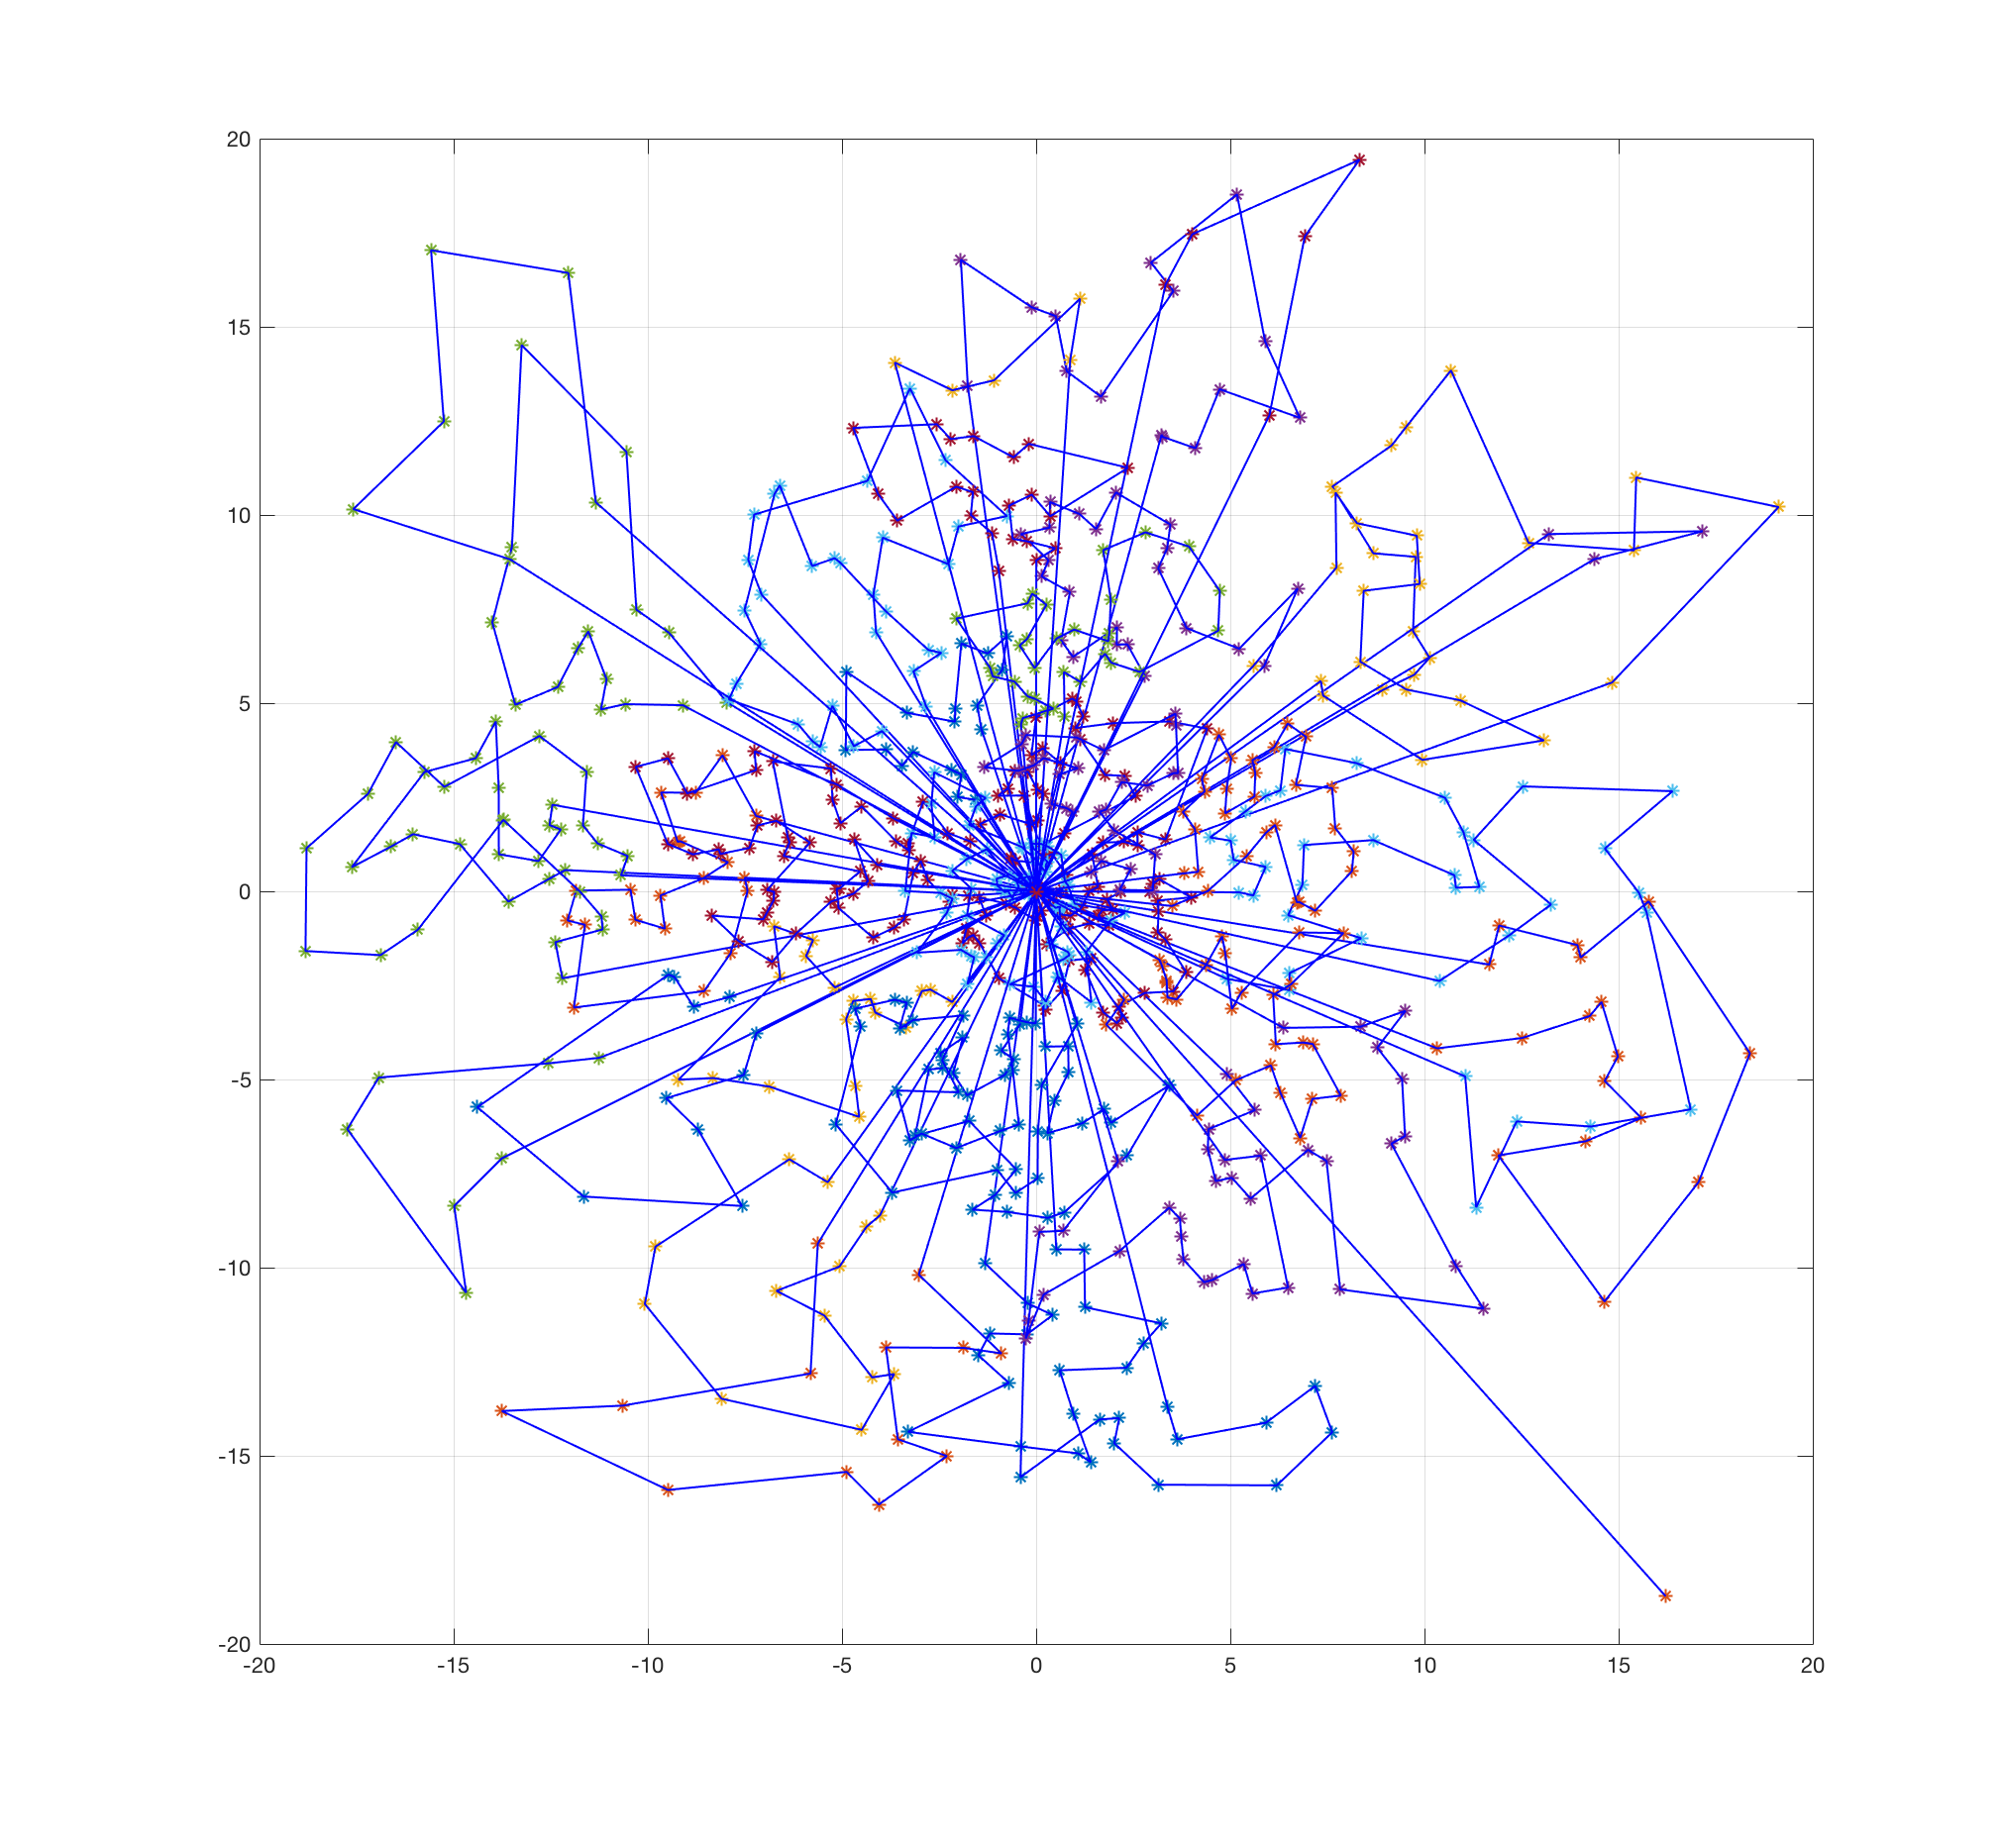
\includegraphics[scale=0.08]{Figs/uav8000_2.png}             
		\end{minipage}}
		%
		%第3张子图
		\subfigure[]{                    
		\begin{minipage}{5cm}
		\centering                        %子图居中
		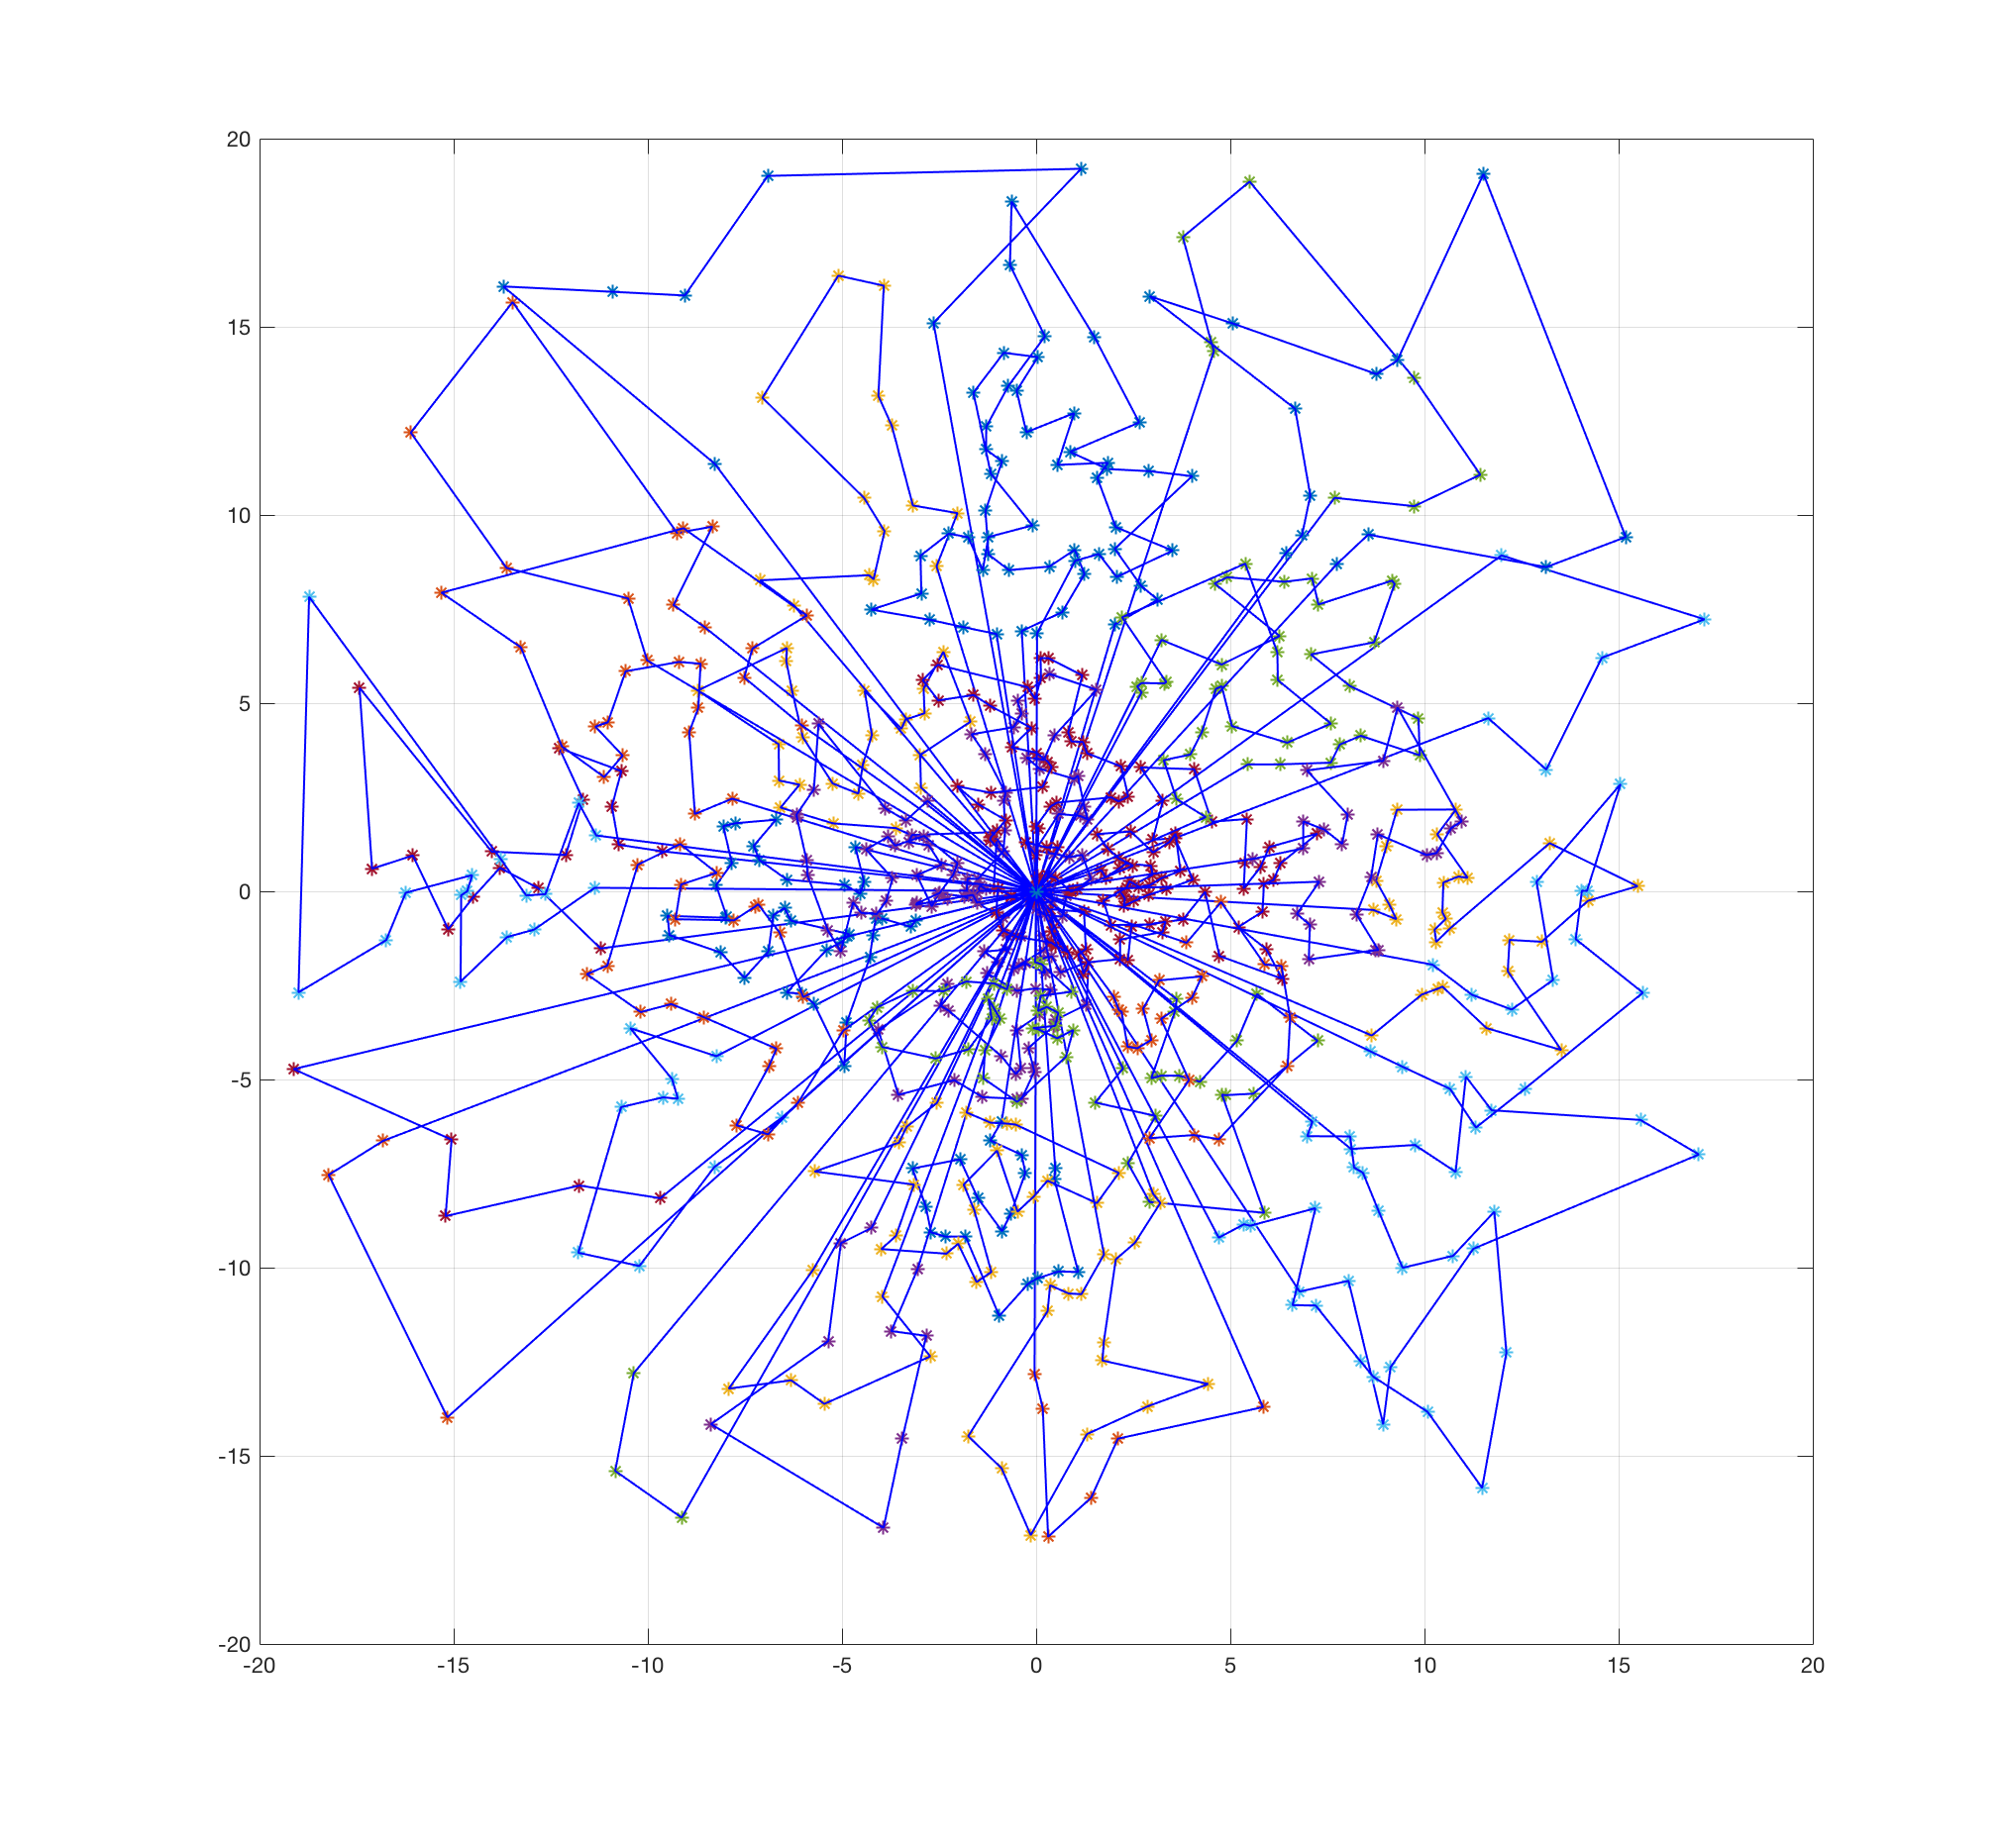
\includegraphics[scale=0.08]{Figs/uav8000_3.png}             
		\end{minipage}}
		% %
		% %第4张子图
		% \subfigure[]{                    
		% \begin{minipage}{6cm}
		%   \centering                        %子图居中
		%   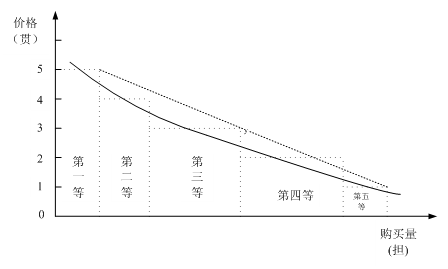
\includegraphics[scale=0.4]{Figs/01.png}             
		% \end{minipage}}
		%                                           
		%大图名称
		\caption{包裹量$N$为8000时,不同随机产生数据下动态规划路线结果图(3幅)} 
		\label{fig:4}                                          %图片引用标记

	\end{figure*}

	\begin{figure*}[!h]

		\centering                                             %居中
		\subfigure[包裹量$N$为1000]{                                          %第一张子图
		\begin{minipage}{7cm}
			\centering                                           %子图居中
			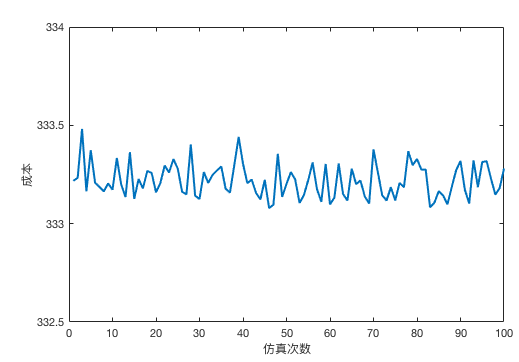
\includegraphics[scale=0.4]{Figs/cost_1000.png}             
		\end{minipage}}
		%
		%第二张子图
		\subfigure[包裹量$N$为8000]{                    
		\begin{minipage}{7cm}
			\centering                        %子图居中
			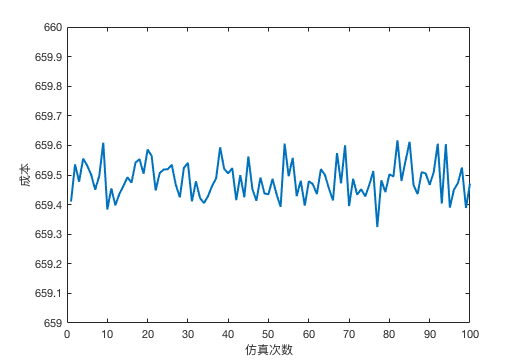
\includegraphics[scale=0.4]{Figs/cost_8000.png}             
		\end{minipage}}
		%                                      
		%大图名称
		\caption{100次随机产生数据下成本值$C(N,T,M)$} 
		\label{fig:5}                                          %图片引用标记

	\end{figure*}














	\subsection{K-Means聚类分配算法}

	针对一块区域内的无人机数量最小问题,通过K-means聚类的思想\citeBUAA{Bahmani:2012tp},将问题转化为最少簇聚类问题,即每一簇的分配的派送任务恰好符合无人机最大性能。因为派送任务的特殊性,不同无人机负责对应区域内的任务能更加高效的完成子任务,从而完成整体区域派送任务。运用K-Means聚类来实现派送区域的分块,K-Means算法接受参数 $k$,将事先输入的n个需要派送的坐标数据划分为 k个簇,使得所获得的聚类满足:(1)同一聚类中的对象相似度较高;(2)而不同聚类中的对象相似度较小。
	%

	在此模型中,改进K-Means中样本与样本之间的欧氏距离,将归一化的权值对原欧氏距离进行加权。根据需要派送区域的经纬度坐标数据$\{X_{1},X_{2},...,X_{n}\}$,从中随机选取k个数据作为初始迭代的聚类中心,同一个K簇聚类会随机选取多次从而迭代选取误差最小的结果。

	迭代下面过程直到收敛:

	1. 对于每一个样例i,计算其应该属于的类
	\begin{eqnarray}
		C_{i}:=\arg \min _{j}\overline {W^{\left( i\right) }}\cdot \left\| x_{i}-\mu _{j}\right\| ^{2}
	\end{eqnarray}

	2. 对于每一个类j,重新计算该类的质心
	\begin{eqnarray}
		\mu _{j}:=\frac {\sum ^{m}_{i=1}1\left\{ C_{i}=j\right\} x_{i}}{\sum ^{m}_{i=1}1\left\{ C_{i}=j\right\} }
	\end{eqnarray}
	%
	%
	%











	\subsection{基于遗传算法的TSP模型}
	当确定无人机的数目和分配的派送任务后,求解最优派送路径问题可以将其看成以TSP问题,即旅行商问题\citeBUAA{Hoffman:2001el}(Travelling Salesman Problem,TSP)。旅行问题是指,有一个旅行商人要拜访n个城市,他需要选择路径必须经过每个城市,并且每个城市的访问次数有且仅有一次,最后还需要返回到起点。无人机派送任务的坐标数据可以映射到连通图,其最优路径的求解可以映射成最小欧拉回路,即TSP问题\citeBUAA{Moon:2002fk}。路径选择的目标函数为所有路径权值之和。派件区域坐标列表:$C = \{c_{1}:1,c_{2}:2,c_{3}:3,...,c_{n}:n\}$,可行解为$T = [t_{1},t_{2},t_{3},...,t_{n}]$。

	遗传算法随机生成一定数量的可行解,并对可行解编码,将问题空间转换为编码空间\citeBUAA{Deb:2000en}。并运用交叉、变异等算子改变解的适应值,以适应性高低作为是否进入下一轮迭代的标准。当适应值越高进入下一轮迭代的概率就越大,也代表在其TSP路径权值之和越小。其中解的适应值:
	\begin{eqnarray}
		fitness\left( T\right) &=&\frac {1}{cost\left( T\right) }\\
		&=&\frac {1}{\min \left( \sum W_{t_{i}t_{i+1}}+W_{t_{n}t_{1}}\right) }
	\end{eqnarray}

	采用轮转式选择样本,轮转式选择也叫做轮盘赌选择,对于种群数为pop size的种群:
	\begin{eqnarray}
		p_{i}=\frac {\sum ^{i}_{s=1}f_{s}}{\sum ^{N}_{j=1}f_{j}}
	\end{eqnarray}

	TSP编码方式是对于目标点集W,假设无人机对各个点的探测序为$G=\{g_{1},g_{2},g_{3},...,g_{n}\}$。每访问一个目标点, 就从点集W中将该点去掉,则第i个所探测的点$g_{i}$在所有未访问点集$W\{g_{1},g_{2},g_{3},...,g_{i-1}\}$中对应的位置序$p_{i}$就可表示所勘测的点, 便利完W中所有的城市。将全部顺序排$p_{i}$在一起得到个序列$P=\{p_{1},p_{2},p_{3},...,p_{n}\}$即表示一条无人机实际的探测路线,即为遗传算法中的一个体。这样编码下的交叉和变异算子是满足编码空间的完备性的。

	因为对于不同数量的坐标信息进行TSP求解,需要根据数据量的大小来设定最大迭代次数,式(8)。
	\begin{eqnarray}
		Gen\left( n\right) &=&a\cdot \log \left( n+b\right) +c\cdot n
	\end{eqnarray}
	其中$n$为每次处理包裹量;$a,b,c$为待定系数。
	%
	%
	%
	%












	\subsection{成本分析模型}
	每个快递站点每小时的快递量是独立同分布的,所以其数量应该服从泊松分布。因此根据设定每次处理包裹量$N$,可以求得无人机最小分配数量$M$、该批次所需要的时间$T$。本文建立成本分析模型来评估规划结果的优劣程度,式(9),最小分配数量$M$和需要的时间$T$与$C(N,T,M)$成正比;每次处理包裹量$N$与$C(N,T,M)$成反比。所以$C(N,T,M)$越高,其规划结果越差,反之则越好。
	\begin{eqnarray}
		C\left( N,T,M\right) &=& -E_{N} \overline N +E_{T}  \overline T+E_{M}  \overline M \\
		\overline N &=& \frac {N}{N_{\max }}\\
		\overline T &=& \frac {T}{T_{\max }}\\
		\overline M &=& \frac {M}{M_{\max }}
	\end{eqnarray}

	其中$E_{N}$、$E_{M}$、$E_{T}$分别为每次处理包裹量$N$、最小分配数量$M$和需要的时间$T$在$C(N,T,M)$权值的期望;$\overline N$、$\overline M$、$\overline M$为每次处理包裹量$N$、最小分配数量$M$和需要的时间$T$的归一化结果。
	%
	%
	%
	%
















	\section{仿真实验和结果分析}

	\subsection{实验一:成本分析}
	建立仿真派送任务,根据真实情况将生成的数据服从于采样得到的近似分布,即包裹的数量$X_{1}$服从于高斯分布,$X_{1} \sim N(10,4)$;包裹的体积$X_{2}$服从于高斯分布,$X_{2} \sim N(3,2) $;包裹的重量$X_{3}$服从于高斯分布,$X_{3} \sim N(1,2)$;正向或逆向物流$X_{4}$服从于二项分布,$X_{4} \sim b(X_{1},0.8)$。

	\begin{figure}
		\centering
		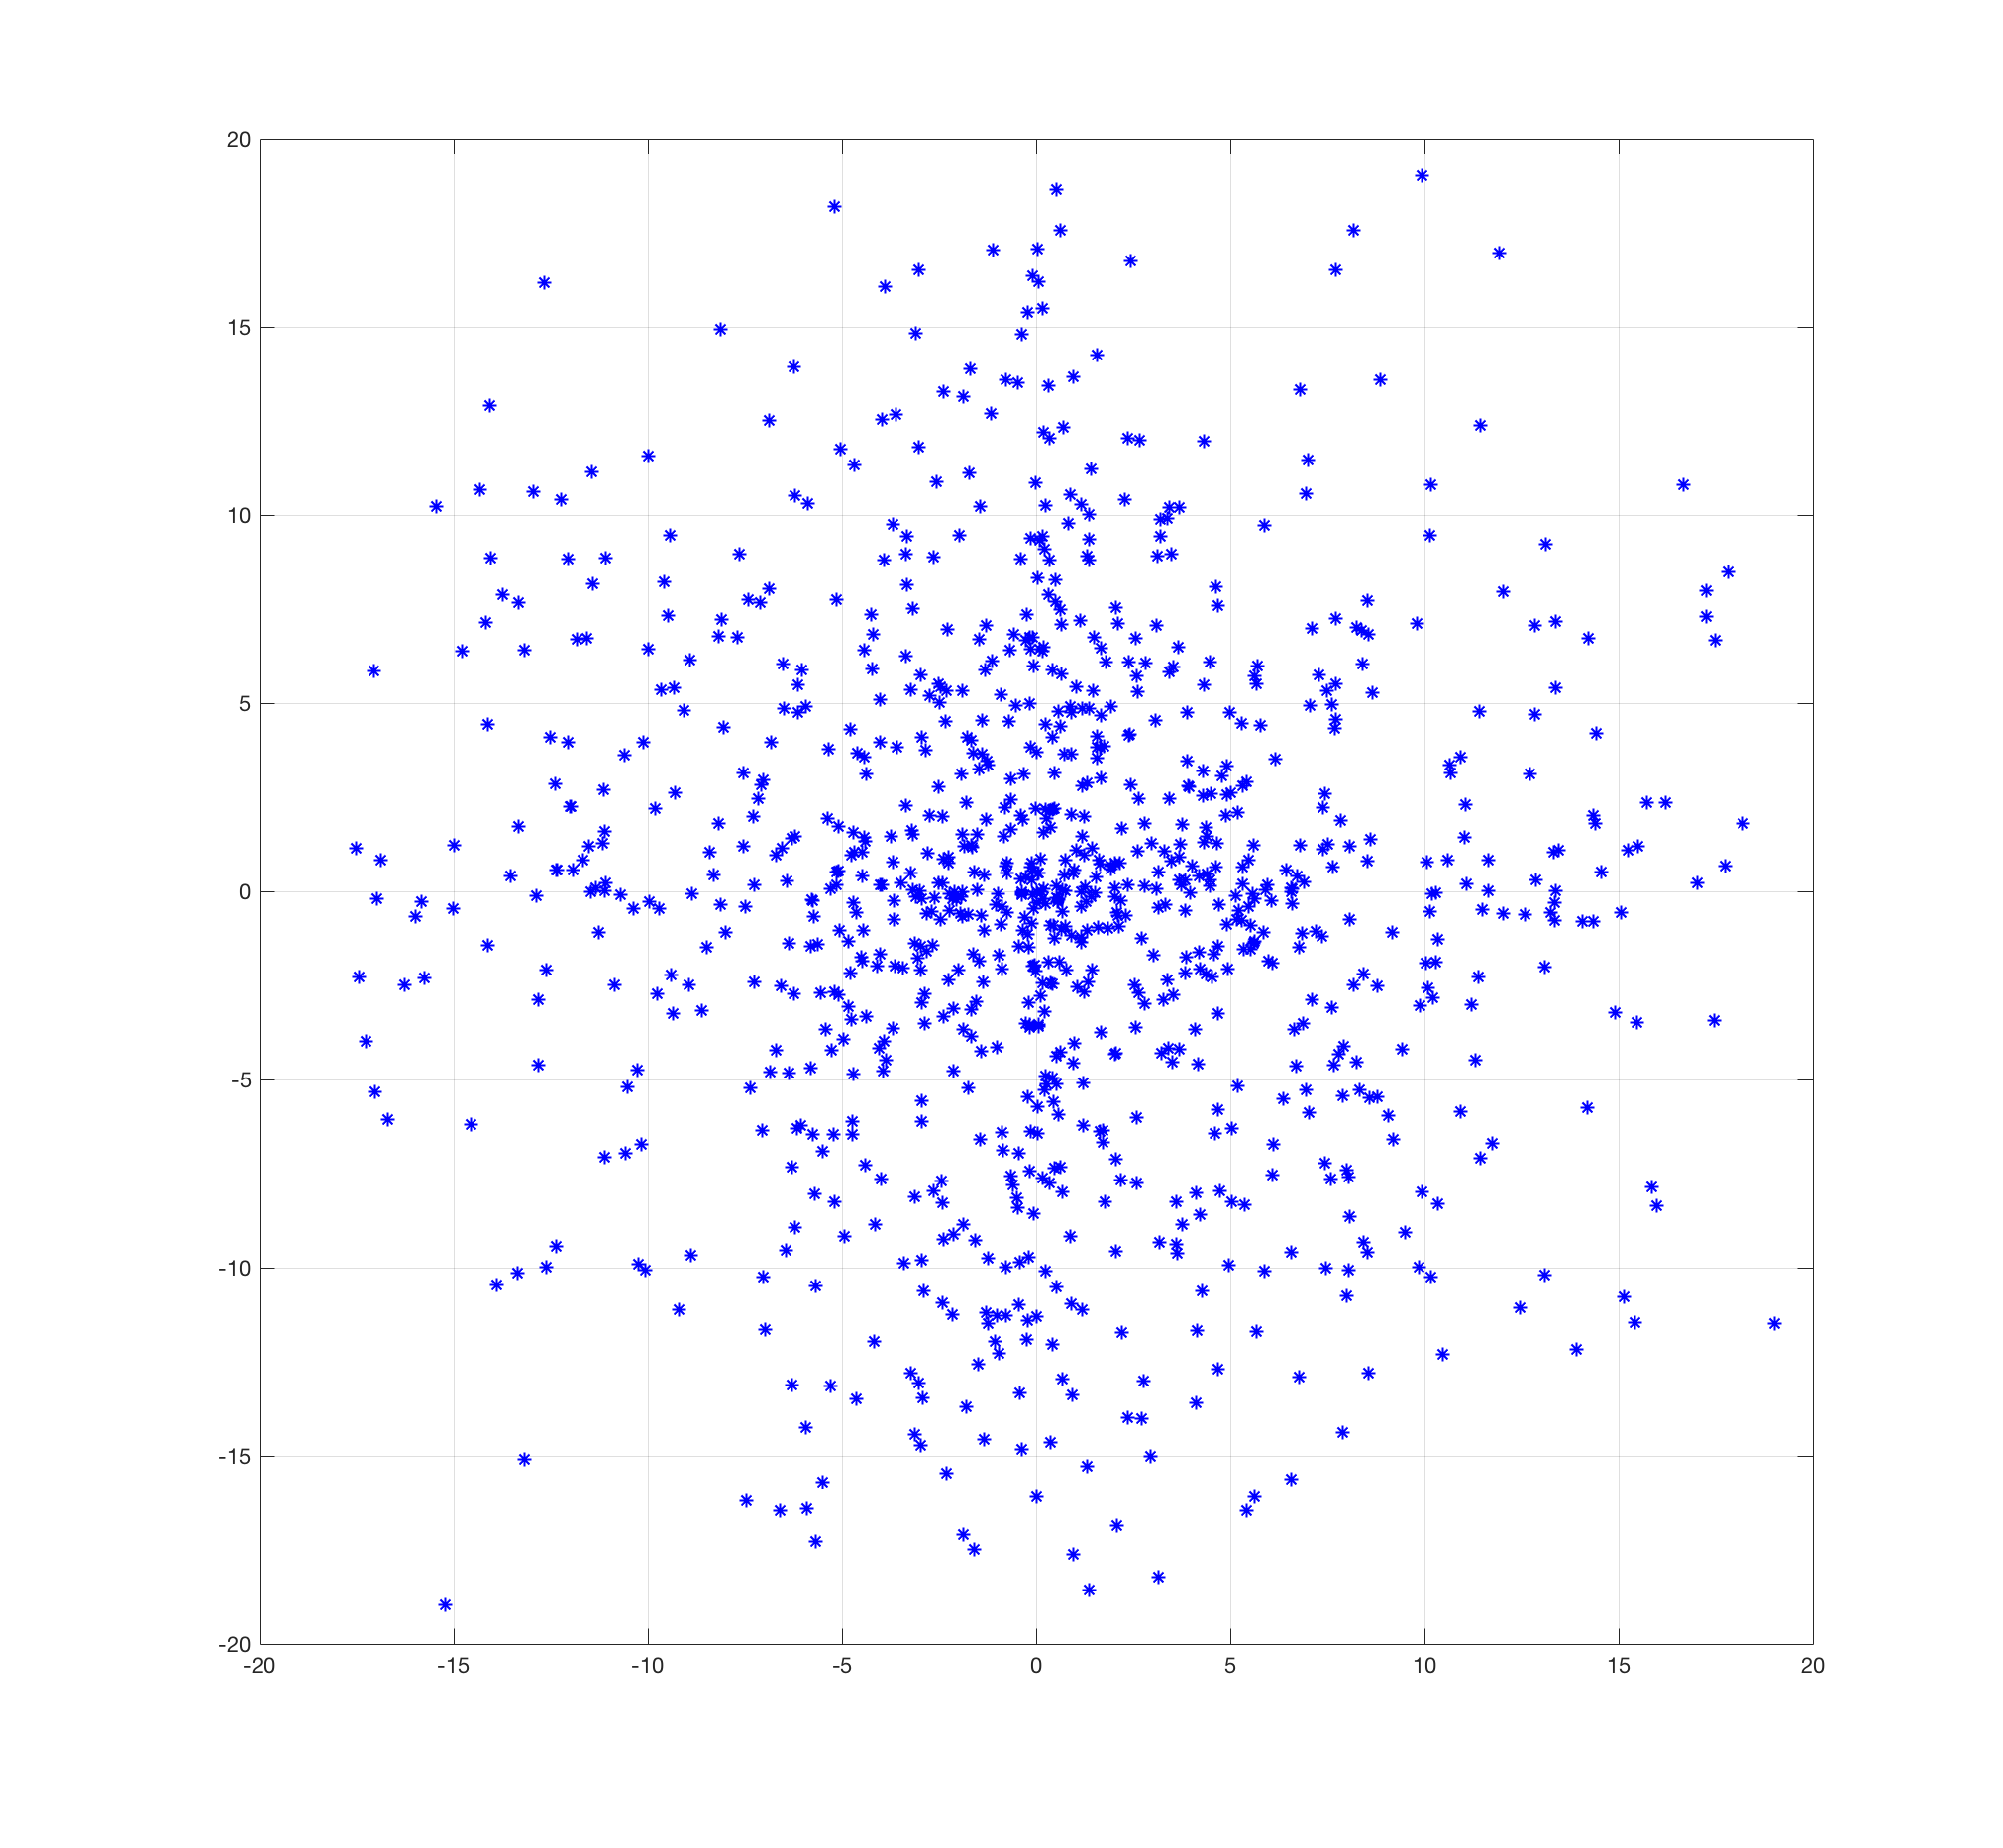
\includegraphics[scale=0.11]{Figs/uavbefore.png}
		\caption{包裹量$N$为10000时,随机产生数据结果图}
		\label{fig:01}
	\end{figure}

	在生成数据后对其进行加权K-Means聚类,将数据分块化。聚类过程中除了加权路径权值之和达到最小的同时,也要考虑最大权值簇小于无人机的最大机能。可以得到对应的结果如图2,取路径之和最大的簇作为此次派送任务的执行时间。

	\begin{figure}
		\centering
		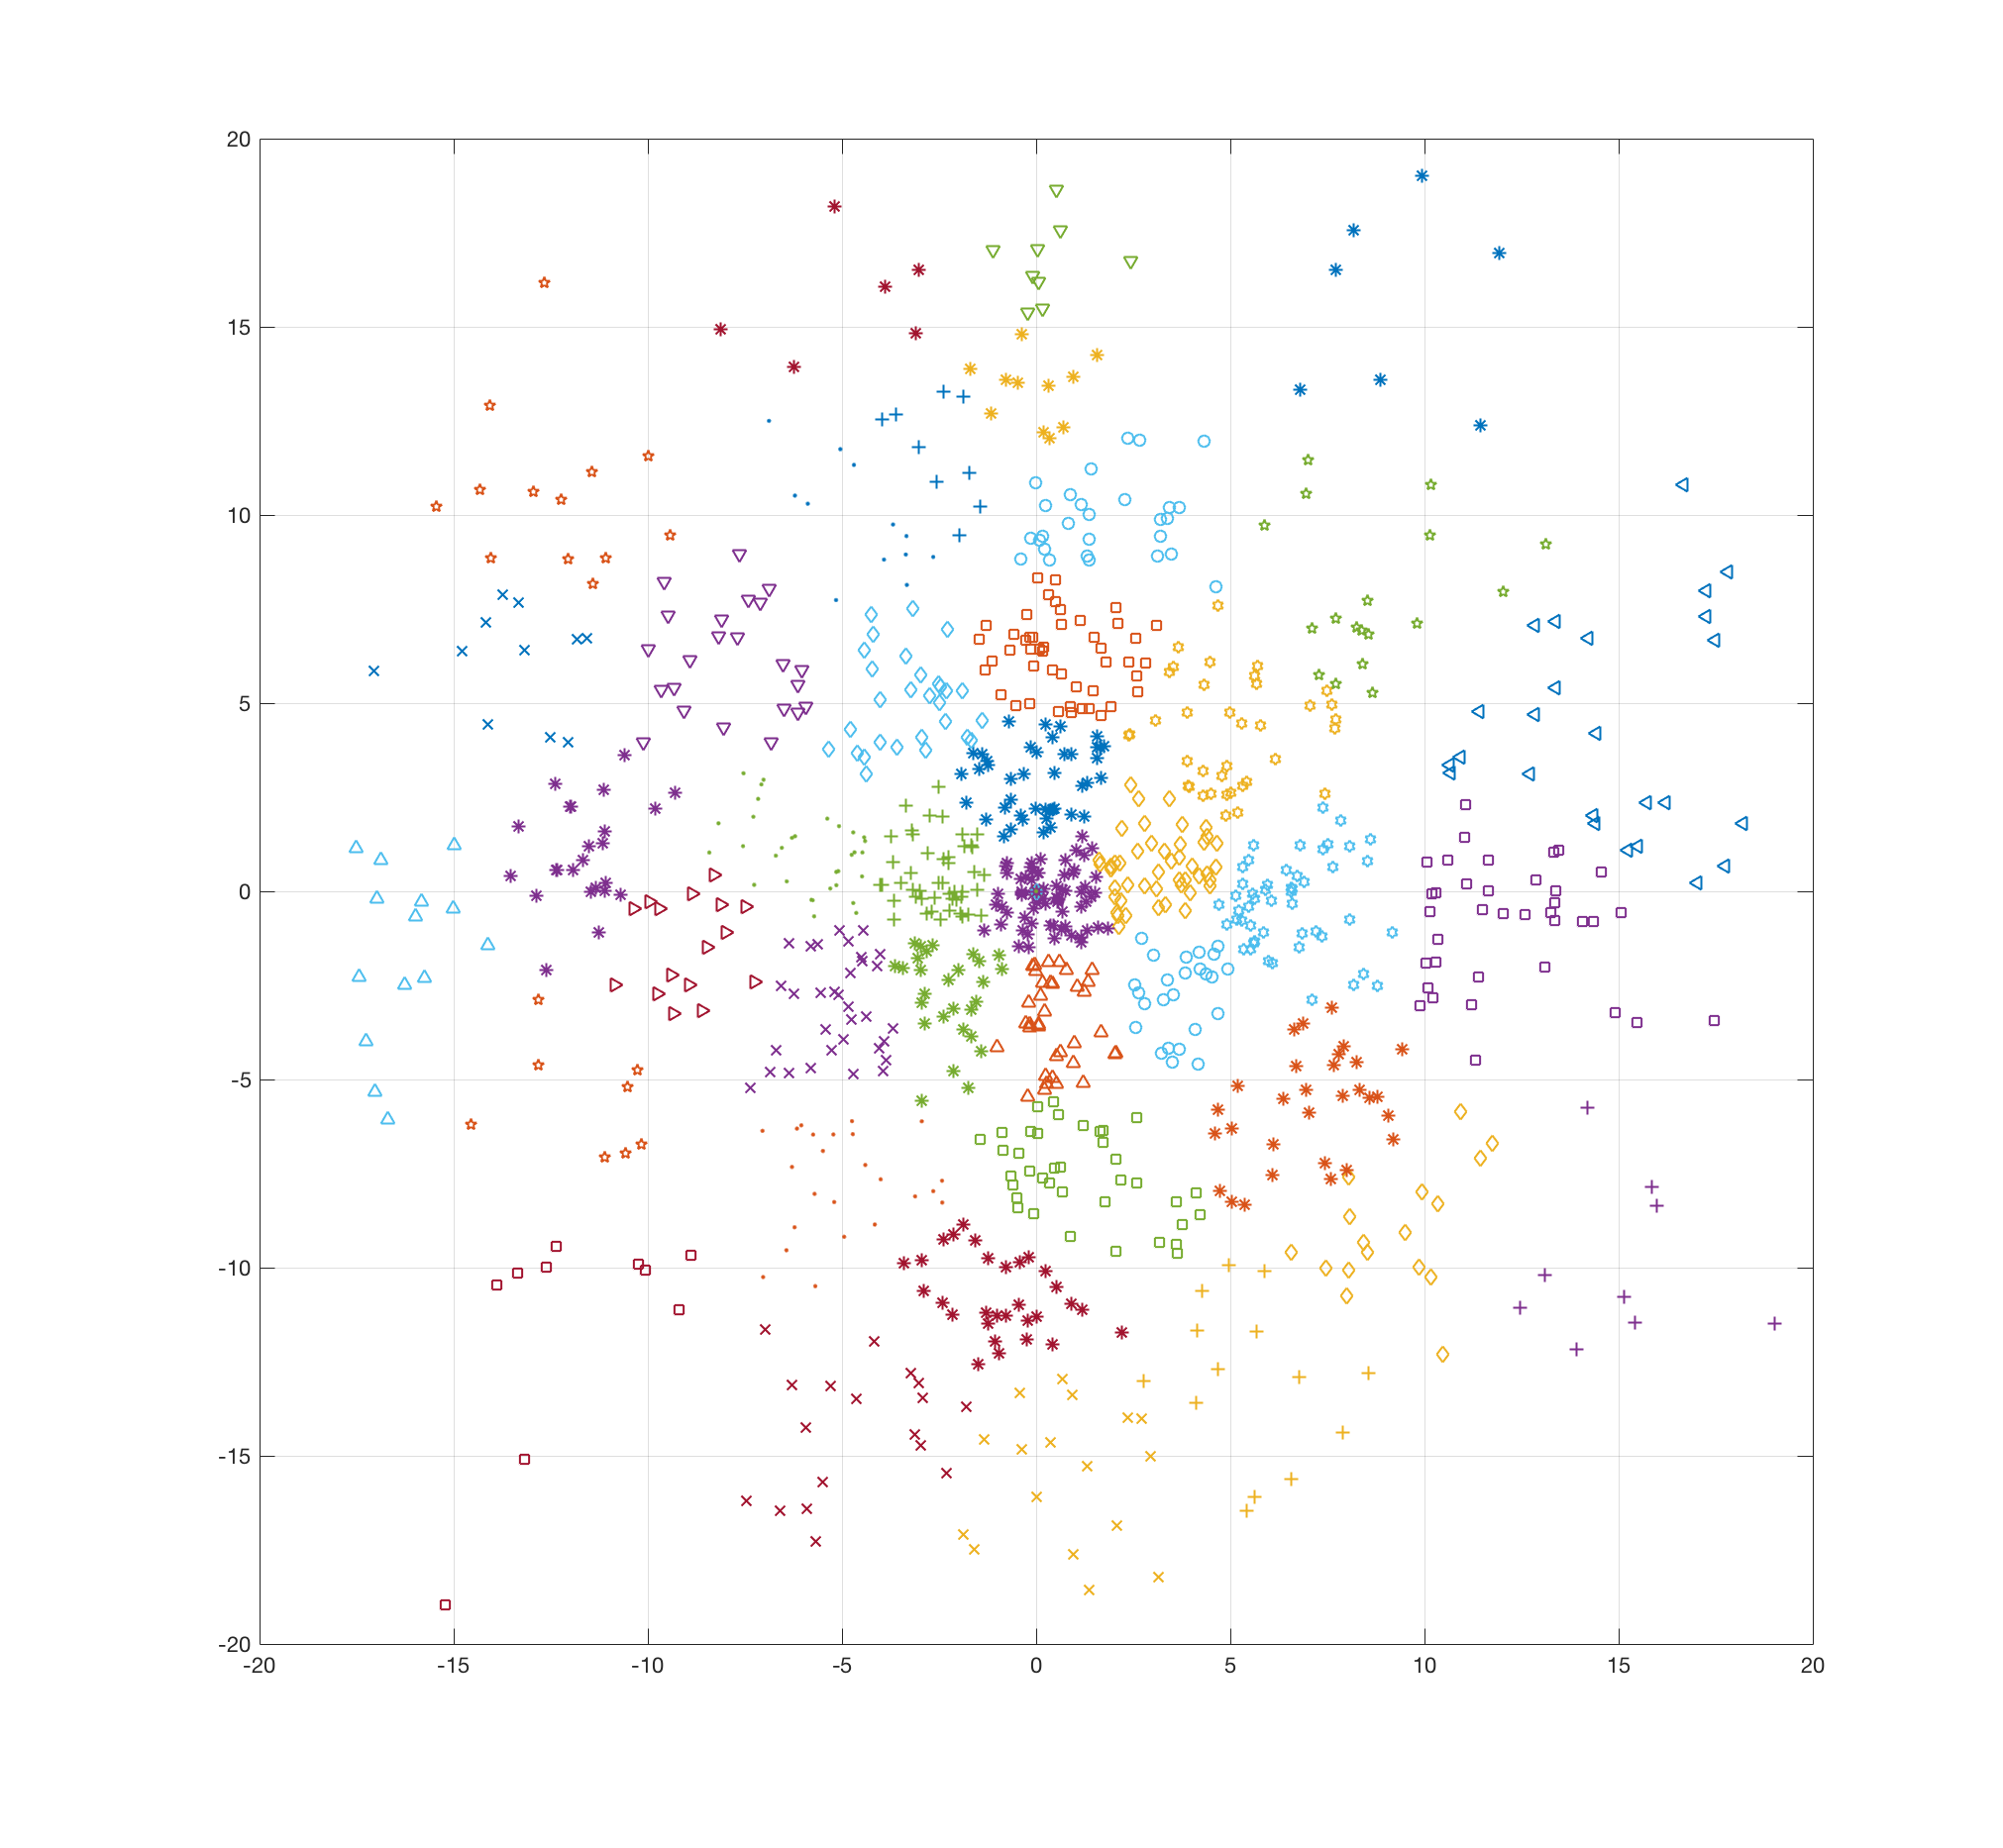
\includegraphics[scale=0.11]{Figs/uavAfter.png}
		\caption{包裹量$N$为10000时,聚类结果图}
		\label{fig:02}
	\end{figure}



	为了避免仿真结果的偶然性,基于每一个包裹量$N$生成的特征数据,将重复进行100次路径规划,最终求得该数值下的平均成本值$C(N,T,M)$。包裹量$N$的定义域设置为$[1000,10000]$,以步长1000取值,即共十个值。因为篇幅有限,本文仅展示$N$为1000和8000的$C(N,T,M)$结果,如图2、图4所示。在图1和图3中,展示随机100次仿真实验中3次的规划路径效果图。图中原点H(0,0)为假设的快递派送中心,即无人机的起点和终点。

	\begin{figure}[!h]
	\centering
	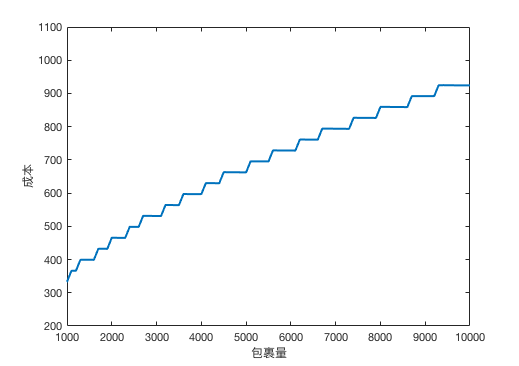
\includegraphics[scale=0.4]{Figs/uavResult.png}
	\caption{包裹量$N$与平均成本值$C(N,T,M)$关系走势图}
	\label{fig:06}
	\end{figure}

	根据图6结果,不难发现在纵坐标包裹量$N$有明显间断性递增趋势。因为在当前数量下无人机的机能必定不能全部发挥,所以存在阈值使得在某一范围内随着包裹量$N$的上升,依旧能完成派送任务,即无需增加无人机的数量。因此在该阈值区间内,成本不会出现明显的提升,甚至因为派送效率的提高而减少成本值。并且随着包裹量$N$的不断变大,该区间范围也同时变大,所以在根据真实派送任务时,可以通过仿真训练找到最适合企业当前业务量的最佳派送包裹量$N$。此外,从图6中还可以看出成本值$C(N,T,M)$与包裹量$N$的斜率小于0.5,即成本值$C(N,T,M)$的增长速率小于包裹量$N$。所以本文动态规划模型可以避免突发包裹量的提升而导致成本值急剧增长。
















	\subsection{实验二:成本对比}
	根据国内物流状况,目前针对于逆向物流采取独立方式进行处理。为了与本文规划模型作对比,以目前国内独立处理的方式建立另一模型,做结果分析。参照目前国内独立方式,本文对比模型采用正向物流和逆向物流独立配送方式,其成本结果$C(N,T,M)$与本文模型作对比,如图7。在图8中,纵坐标是两结果之差,横坐标是包裹量$N$。不难发现随着包裹量$N$不断增大,两者成本之差显著上升。

	\begin{figure}[!h]
	\centering
	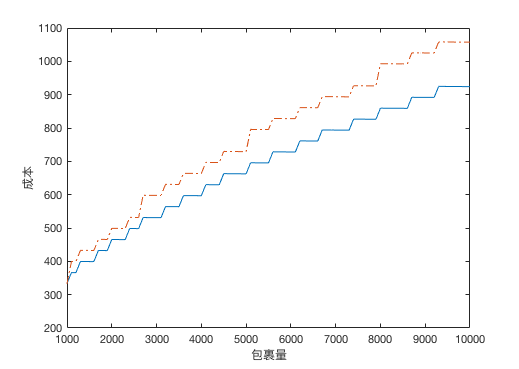
\includegraphics[scale=0.4]{Figs/compare.png}
	\caption{对比图}
	\label{fig:07}
	\end{figure}

	\begin{figure}[!h]
	\centering
	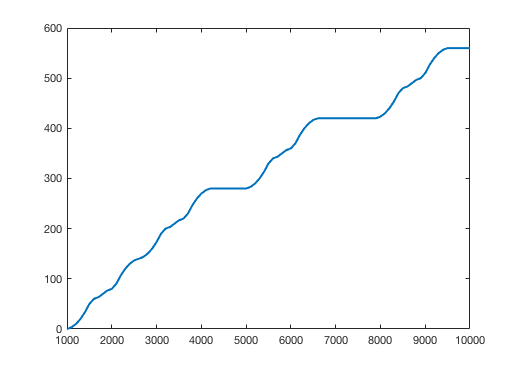
\includegraphics[scale=0.4]{Figs/compare2.png}
	\caption{差值对比图}
	\label{fig:08}
	\end{figure}












	%%%%%%%%%%%%%%%%%%%%%%%%%%%%%%%%%%%%%%%%%%%%%%%%%%%%%%%%%%%%%%%%
	%  参考文献
	%%%%%%%%%%%%%%%%%%%%%%%%%%%%%%%%%%%%%%%%%%%%%%%%%%%%%%%%%%%%%%%%

	\renewcommand\refname{\hei\wuhao\centerline{参考文献(References)}\global\def\refname{参考文献}}
	\vskip 12pt

	\let\OLDthebibliography\thebibliography
	\renewcommand\thebibliography[1]{
		\OLDthebibliography{#1}
		\setlength{\parskip}{0pt}
		\setlength{\itemsep}{0pt plus 0.3ex}
	}

	{
		\renewcommand{\baselinestretch}{0.9}
		\liuhao
		\bibliographystyle{unsrt}
		%bib文件名字
		\bibliography{uav}
	}
  
\end{document}
